\documentclass{article}\usepackage[]{graphicx}\usepackage[]{color}
%% maxwidth is the original width if it is less than linewidth
%% otherwise use linewidth (to make sure the graphics do not exceed the margin)
\makeatletter
\def\maxwidth{ %
  \ifdim\Gin@nat@width>\linewidth
    \linewidth
  \else
    \Gin@nat@width
  \fi
}
\makeatother

\definecolor{fgcolor}{rgb}{0.345, 0.345, 0.345}
\newcommand{\hlnum}[1]{\textcolor[rgb]{0.686,0.059,0.569}{#1}}%
\newcommand{\hlstr}[1]{\textcolor[rgb]{0.192,0.494,0.8}{#1}}%
\newcommand{\hlcom}[1]{\textcolor[rgb]{0.678,0.584,0.686}{\textit{#1}}}%
\newcommand{\hlopt}[1]{\textcolor[rgb]{0,0,0}{#1}}%
\newcommand{\hlstd}[1]{\textcolor[rgb]{0.345,0.345,0.345}{#1}}%
\newcommand{\hlkwa}[1]{\textcolor[rgb]{0.161,0.373,0.58}{\textbf{#1}}}%
\newcommand{\hlkwb}[1]{\textcolor[rgb]{0.69,0.353,0.396}{#1}}%
\newcommand{\hlkwc}[1]{\textcolor[rgb]{0.333,0.667,0.333}{#1}}%
\newcommand{\hlkwd}[1]{\textcolor[rgb]{0.737,0.353,0.396}{\textbf{#1}}}%

\usepackage{framed}
\makeatletter
\newenvironment{kframe}{%
 \def\at@end@of@kframe{}%
 \ifinner\ifhmode%
  \def\at@end@of@kframe{\end{minipage}}%
  \begin{minipage}{\columnwidth}%
 \fi\fi%
 \def\FrameCommand##1{\hskip\@totalleftmargin \hskip-\fboxsep
 \colorbox{shadecolor}{##1}\hskip-\fboxsep
     % There is no \\@totalrightmargin, so:
     \hskip-\linewidth \hskip-\@totalleftmargin \hskip\columnwidth}%
 \MakeFramed {\advance\hsize-\width
   \@totalleftmargin\z@ \linewidth\hsize
   \@setminipage}}%
 {\par\unskip\endMakeFramed%
 \at@end@of@kframe}
\makeatother

\definecolor{shadecolor}{rgb}{.97, .97, .97}
\definecolor{messagecolor}{rgb}{0, 0, 0}
\definecolor{warningcolor}{rgb}{1, 0, 1}
\definecolor{errorcolor}{rgb}{1, 0, 0}
\newenvironment{knitrout}{}{} % an empty environment to be redefined in TeX

\usepackage{alltt}

\usepackage{fullpage}

\usepackage{color}
\usepackage[dvipsnames,svgnames,table]{xcolor}

\usepackage{wrapfig,float}
\usepackage{caption}
\usepackage{subcaption}
\usepackage{graphicx}
\usepackage{sidecap}

\usepackage{multirow}
\usepackage{multicol}
\usepackage{rotating}

\usepackage{amssymb}
\usepackage{amsmath}
\usepackage{bbm}

\usepackage{natbib}
\bibliographystyle{apa}
\usepackage[utf8]{inputenc} % allows UTF8 chars in bib file

\usepackage{url}
\usepackage[pdftex,hypertexnames=false,linktocpage=true]{hyperref}
\hypersetup{colorlinks=true,linkcolor=blue,anchorcolor=blue,citecolor=blue,filecolor=blue,urlcolor=blue,bookmarksnumbered=true,pdfview=FitB}

\usepackage[colorinlistoftodos]{todonotes}

% Todo commands
\newcommand{\done}[2][inline]{\todo[color=SpringGreen, #1]{#2}}
% for todos that have been seen and dealt with
\newcommand{\meh}[2][inline]{\todo[color=White, #1]{#2}}
% for todos that may no longer be relevant
\newcommand{\comment}[2][inline]{\todo[color=SkyBlue, #1]{#2}}
% for comments that may not be "to-do"s
\newcommand{\mcomment}[1]{\todo[color=SkyBlue]{#1}}
% for margin comments
\newcommand{\newtext}[1]{\todo[inline, color=White]{ \color{OliveGreen}{#1}}}
% new text - not necessarily something to be done
\newcommand{\move}[1]{\todo[inline, color=Lime]{#1}}
% new to do item

\title{Perception and Cognition in Statistical Graphics}
\author{Susan VanderPlas}
\IfFileExists{upquote.sty}{\usepackage{upquote}}{}
\begin{document}

\graphicspath{{Figure/}{Images/}}

\maketitle




Statisticians produce graphics for a multitude of reasons: to understand the structure of raw data, to check model assumptions, to present model predictions in an informative fashion; all of these goals are facilitated by appropriate visualizations. Some of these goals are best served by quick-and-dirty representations of the data, while highly polished graphics may be more useful for other goals. Regardless, it is important to convey the data appropriately, which means we must understand how graphics are perceived on at least a basic level. Tukey focused on graphics as a tool for exploratory analysis, because pictures can often display the data in a more coherent fashion than a table or spreadsheet; his book, \citet{eda} details many different types of graphics and the appropriate situations to utilize them. This chapter focuses on the interaction between graphics and the human visual system, with the goal of understanding how  to most efficiently and effectively convey information using statistical graphics. We will first consider the physiology and psychology of the perceptual experience in general, and then address the issue of graph-specific perception.

\section{The Human Visual System}
In order to design graphics for the human perceptual system, we must understand, at a basic level, the makeup of the perceptual system. There are multiple levels of perception that must correctly function in order to perceive visual stimuli successfully, but a somewhat simplistic higher-level analogy would be that we must understand both the hardware and software of the human visual system to create effective graphics.

The ``hardware", in this analogy, consists of the neurons that make up the eyes, optic nerve, and the brain itself. The higher-level functions (object recognition, working memory, etc.) comprise the ``software" component. In addition, much like computer software, there are different programs running simultaneously; these programs may interact with each other, run sequentially, or run in parallel. The following sections provide an overview of the grey-matter (hardware) components of the visual system as well as the higher-level cognitive heuristics (software) that order the raw input and construct our visual environment.

\subsection{Hardware}
The physiology of perception is complex; what follows is a brief overview of the physiology of perception, focusing on the areas most important to the perception of statistical graphics. This physiological information is important in understanding the difference between the sensation (i.e. the retinal image) and the perception (the corresponding mental representation), which is an important distinction in understanding how statistical graphics are perceived. This overview will entirely ignore the finer details of the organization of the brain: feature detector cells, specific processing units for certain types of visual stimuli, and most of the horrifying or amusing experiments and incidents that led to the understanding of the brain. A more thorough presentation of these aspects of perception can be found in \citet{goldstein}.

\paragraph{The Eye}
The eye is a complex apparatus, but for our purposes, the most important component of the eye is the retina, which contains the sensory cells responsible for transforming light waves into electrical information in the form of neural signals. These sensory cells are specialized neurons, known as rods and cones, which perceive light intensity (brightness) and wavelength (color), respectively. One section of the retina, known as the fovea, contains only cones; the rest of the retina contains a mixture of rods and cones. Figure \ref{fig:retina} depicts the structure of the eye with a closeup of the retina.

\begin{figure}
\centering
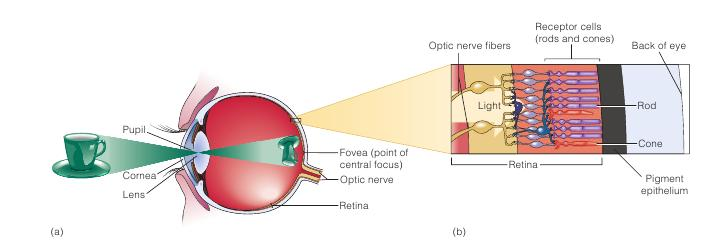
\includegraphics[width=.8\linewidth, keepaspectratio=TRUE]{Retina}
\caption[The human eye, with closeup of receptor cells in the retina]{The human eye, with closeup of receptor cells in the retina (image from \protect\citealt{goldstein}, chap 3.1).} \label{fig:retina}
\end{figure}

Another important region of the retina is the blindspot, the area where the optic nerve exits the eye to connect the retina to the brain. There are no rods or cones in this region of the retina, and any vision in the region of space that maps onto this point is a result of two mechanisms: binocular vision (the other eye fills in the missing information) and your brain ``filling in" what it believes should be there.

\begin{figure}[htbp]\centering
\begin{center}
\fbox{
\begin{minipage}[c]{5in}
\vspace{2cm}
\Large
\hfill\textbf{R}\hspace{3in}\textbf{L}\hfill
\vspace{2cm}
\end{minipage}}
\end{center}
\caption[Blind Spot]{Illustration of the blind spot in the retina. Close one eye, and focus the other on the appropriate letter (R if the right eye is still open, L if the left eye is still open). Place the paper approximately 1 foot from your eye, and move the paper toward or away from your face until you notice the other letter disappear. Your brain ``fills in" the other letter with the background.}\label{fig:blindspot}
\end{figure}

Figure \ref{fig:ColorRange} shows the responsiveness of rods and each of the three types of cones to wavelengths of light in the visual spectrum. This image suggests that we have relatively good visual discrimination of the yellow-green portion of the color spectrum, but relatively poor discrimination of colors in the red and blue portions of the color spectrum.

\begin{figure}[htbp]\centering
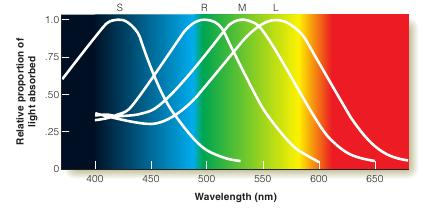
\includegraphics[width=.6\linewidth, keepaspectratio=TRUE]{AbsorptionSpectra}
\caption[Absorption spectra of retinal cells]{Absorption spectra of rods and short, medium, and long wave cones. (image from \protect\citealt{goldstein}, chap 3.3).} \label{fig:ColorRange}
\end{figure}

As a result, rainbow-style color schemes are seldom appropriate for conveying numerical values, because the correspondance between the perceived information and the displayed information is not accurately maintained by the visual system \citep{rainbowcolor}. In addition, if any of the cones are missing or damaged as a result of genetic mutations, color perception is impaired, resulting in a smaller range of distinguishable colors. This set of impairments is known coloquially as color-blindness, and occurs in an estimated 5\% of the population (approximately 10\% of males, and less than 1\% of females). Color blindness is discussed in more depth in section \ref{colorblindness}.

\paragraph{The Brain}
Once light hits the retina and causes a signal in the receptor cells, the information travels along the optic nerve and into the brain. Multiple neighboring rods are connected to the same neuron, where each cone is connected to a single neuron. The combined wiring of rod cells is responsible for the Hermann grid illusion and the Mach bands seen in figure \ref{fig:InhibitionIllusions}. Both of these illusions are a product of lateral inhibition, which is a result of the wiring of rod cells in the retina. Essentially, neurons can only fire at a specific rate, so when neighboring cells are all stimulated simultaneously, the combined neuron cannot fire fast enough to pass on all of the signals, causing ``inhibition". The specifics of this response and its relationship with the wiring of the receptor cells are somewhat complex; a more thorough explanation can be found in \citet{goldstein}, chapter 3.4.

\begin{figure}
\centering
\begin{subfigure}[b]{.45\linewidth}
  \centering
  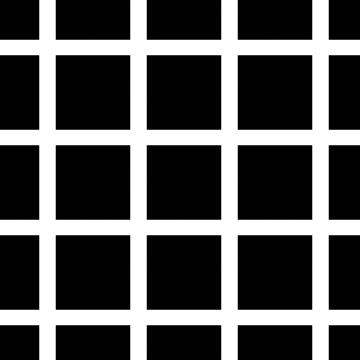
\includegraphics[width=\linewidth]{HermannGrid}
  \caption{\small Hermann Grid Illusion \label{fig:hermanngrid}}
\end{subfigure}\hfill
\begin{subfigure}[b]{.45\linewidth}
  \centering
  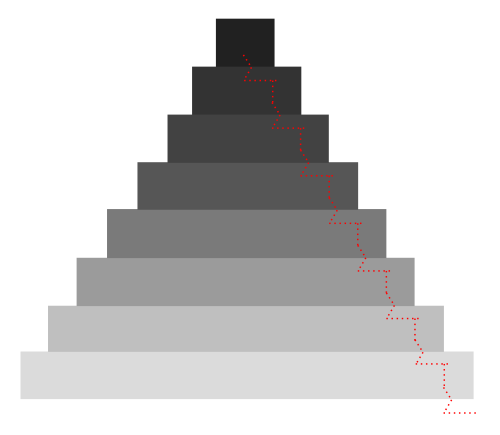
\includegraphics[width=\linewidth]{MachBands}
  \caption{\small Mach Bands.
  \label{fig:machbands}}
\end{subfigure}
\caption[Inhibition Illusions]{Optical Illusions resulting from lateral inhibition. The Hermann Grid illusion causes dark circles to appear at the intersection of white lines; the Mach bands illusion causes the borders of adjacent rectangles to appear more strongly defined.} \label{fig:InhibitionIllusions}
\end{figure}

Once neural impulses have left the retina through the optic nerve, they travel to the visual cortex by way of several specialized structures within the brain that process lower-level signals. Receptor cells in the visual cortex respond to specific angles, spatial locations, colors, and intensities, and arrays of these special 'feature detector cells' process the information into a form that higher-level processes can utilize. These higher-level processes are what we have previously called 'software': they are not directly related to the physical brain, but they do process information heuristically to produce higher-level reasoning and conclusions. In the next section, we explore some of the higher-level processes responsible for visual perception.

\subsection{Software}\label{Software}
Many of the processes for visual perception run simultaneously; in absence of a strict temporal ordering, we will start with the more basic tasks of visual perception and proceed towards higher-level processes. We will begin with attention.

\subsubsection{Attention and Perception} \label{AttentionPerception}
In many tasks, it is necessary to pay attention to many parallel input streams simultaneously; this is particularly true for complex tasks like driving a car. These tasks demand divided attention; the brain must process many different sources of information in parallel. By contrast, most image recognition tasks require selective attention, that is, focusing on specific objects and ignoring everything else. The brain accomplishes this attention through several mechanisms.

Selective attention is accomplished by focusing the fovea (the area with the highest visual acuity) on the object. For instance, if the object is a page of text, each word will pass through the fovea, producing a focused stream of visual input. This stream of input consists of saccades (jumps between points of focus) and pauses in which the visual information is relayed to the brain. Figure \ref{fig:saccadestext} shows the saccades (lines) and pauses (circles) resulting when someone scans a paragraph of text. These saccades and pauses are utilized in eye-tracking technology to determine which parts of an image the observer is focusing on (and by extension, which information is being encoded by the brain). Further discussion of eye tracking is provided in section \ref{experimentalmethods}.

\begin{figure}[htbp]
\centering
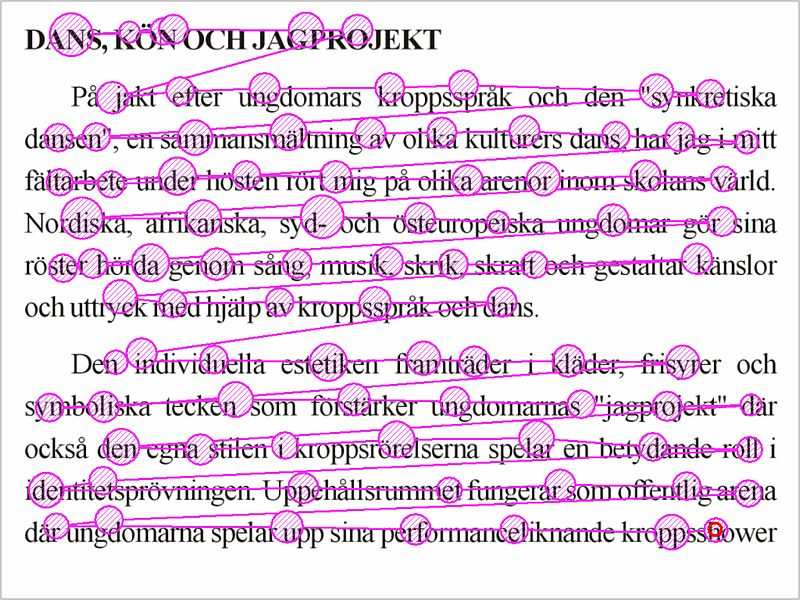
\includegraphics[width=.5\linewidth]{SaccadesText}
\caption[Saccades and Pauses]{A plot of saccades made while reading text. Saccades, shown by the lines, indicate ``jumps", while pauses are shown by circles, with size proportional to the time spent focusing on that area.}\label{fig:saccadestext}
\end{figure}

Selective attention is generally necessary for perception to occur, though there is some information that is encoded automatically. Experiments such as the fairly famous \href{http://www.theinvisiblegorilla.com/videos.html}{``gorilla" film}\footnote{\url{http://www.theinvisiblegorilla.com/videos.html}} demonstrate that even when there is attention focused on a task, information extraneous to that task is not always encoded, that is, even when participants focused on counting the number of passes between players in the basketball game, they did not notice the gorilla walking through the middle of the court. It is important to understand which parts of a visual stimulus are the focus of a given perceptual task, because most of the information encoded by the brain is a result of selective attention. Eye-tracking can be an important tool useful to understand these perceptual processes, but participants are often able to report which parts of a stimulus contributed to their decision as well.

Within the brain, attention is important because it allows different regions of the brain which process color, shape, and position to integrate these perceptions into a multifaceted mental representation of the object \citep{goldstein}. This process, known as binding, is essential to coherently encode a scene into working memory. Feature integration theory \citep{treisman1980feature} suggests that these separate streams of information are initially encoded in the preattentive stage of object perception; focusing on the object triggers the binding of these separate streams into a single coherent stream of information. Many single features, such as color, length, and texture are \emph{preattentive}, because they can be pinpointed in an image without focused attention (and thus can be located faster), but specific combinations of color and shape require attention (because the features must be bound together) and are thus more difficult to search. Preattentive features are generally processed in parallel (that is, the entire scene is processed nearly simultaneously), while features requiring attention are processed serially. Examples of features processed  serially and in parallel are shown in figure \ref{fig:parallelSerialFeatures}, taken from Chapter 6 of \citet{helander1997handbook}. The importance of preattentive processing to statistical graphics is discussed in Section \ref{LowLevelGraphics}, which includes a demonstration of preattentive search in figure \ref{fig:preattentive}.

\begin{figure}[htbp]\centering
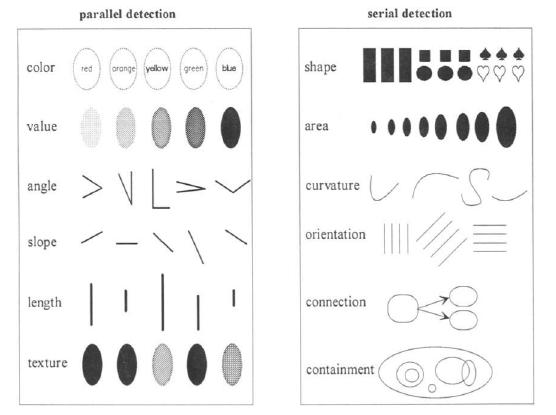
\includegraphics[width=.8\linewidth]{ParallelSerialFeatures}
\caption[Parallel and Serial Feature Detection]{Examples of features detected serially or in parallel (Chapter 6, \protect\citealt{helander1997handbook})}\label{fig:parallelSerialFeatures}
\end{figure}

Feature integration as a result of attention enables the brain to process a figure holistically and integrate all of the separate aspects of the object into a single perceptual experience. This processing is important for the most basic visual processes we take for granted, including object perception.

\subsubsection{Object Perception} \label{ObjectPerception}
The most basic task of the visual system is to perceive objects in the world around us. This is an inherently difficult task, however, because the retina is a flat, two-dimensional surface responsible for conveying a three-dimensional visual scene. This dimensional reduction means that there are multiple three-dimensional stimuli that can produce the same visual image on the retina. This is known as the inverse projection problem - an infinite number of three-dimensional objects produce the same two-dimensional image. Less relevant to statistical graphics, but still complicating the object perception process, a single object can be viewed from a multitude of angles, in many different situations which may affect the retinal image (lighting, partial obstruction, etc). In addition, we recognize objects even when they are partially obscured or viewed from an angle we have not previously seen. These problems mean that the brain must utilize many different heuristics to increase the accuracy of the perceived world relative to an ambiguous stimulus.

The most commonly cited set of heuristics for object perception (and the set most relevant to statistical graphics) are known as the \emph{Gestalt Laws of Perceptual Organization} (\citealt{goldstein}, Chapter 5.2). These laws are related to the idea ``the whole is greater than the sum of the parts'', that is, that the components of a visual stimulus, when combined, create something that is more meaningful than the separate components considered individually. The Gestalt laws are as follows \citep{goldstein}:

\begin{itemize}
\item \textbf{Pragnanz - the law of good figure}. (Also referred to as the law of closure) Every stimulus pattern is seen so that the resulting structure is as simple as possible.
\item \textbf{Proximity}. Things that are close in space appear to be grouped.
\item \textbf{Similarity}. Similar items appear to be grouped together. The law of similarity is usually subordinate to the law of proximity.
\item \textbf{Good Continuation}. Points that can be connected to form straight lines or smooth curves seem to belong together, and lines seem to follow the smoothest path.
\item \textbf{Common Fate}. Things moving in the same direction are part of a single group.
\item \textbf{Familiarity}. Things are more likely to form groups if the groups are familiar.
\item \textbf{Common Region}. Things that are in the same region (container) appear to be grouped together
\item \textbf{Uniform Connectedness}. A connected region of objects is perceived as a single unit.
\item \textbf{Synchrony}. Events occurring at the same time will be perceived as belonging together.
\end{itemize}

\begin{figure}[htbp]\centering
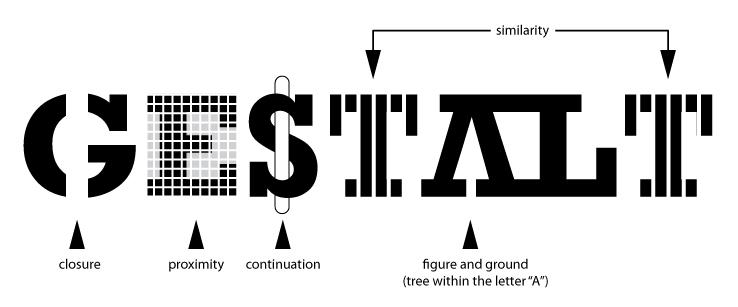
\includegraphics[width=.9\linewidth]{gestalt}
\caption[The gestalt laws of perception]{The gestalt laws of perception \protect\footnotemark}\label{fig:gestaltlaws}
\end{figure}
\protect\footnotetext{From \url{http://yusylvia.files.wordpress.com/2010/03/gestalt_illustration-01.jpg}}
Figure \ref{fig:gestaltlaws} shows examples of many of the gestalt laws, which when combined help to order our perceptual experience. We have discussed how we attend to visual stimuli and how they are recognized, but for the perceptual experience to be meaningful, previous experiences must be stored into memory in some coherent way. The next section discusses how visual scenes are stored into long-term memory.

\subsubsection{Visual Memory}
We have discussed how visual stimuli are perceived and how objects are recognized; we now must examine how visual stimuli are encoded into memory. Most researchers believe that visual perceptions are encoded in an analog fashion, so that the memory of an image is closely related to the perception of that same image \citep{cognition}. Other theories suggest that visual perceptions are encoded semantically, that is, the description of a visual scene would be encoded, rather than a mental ``image" of that scene. Both theories are likely at least partially correct, but the analog encoding of visual images is more relevant to statistical graphics because the accuracy of the stored image has the potential to affect recall of the contents of that image (and thus what people remember about a particular graphic). Experimental evidence for analog encoding includes the mental rotation task, where participants must determine whether or not a figure is a rotation of a target figure, as shown in figure \ref{fig:mentalRotation}. \citet{shepard1988mental} showed that reaction time was proportional to the angle of rotation of the stimuli, which suggests that participants were mentally rotating the figure as they would rotate a three-dimensional figure in space.

\begin{figure}[htbp]\centering
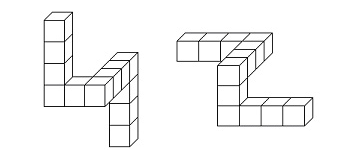
\includegraphics[width=.7\linewidth]{RotationTask}
\caption[Rotation Task]{Rotation task \protect\citep{shepard1988mental}. Are the two images the same?}\label{fig:mentalRotation}
\end{figure}

In addition, \citet{kosslyn1978visual} showed that mental representation of distances in a figure are accurate and that the time to encode those distances is proportional to the distances in the actual figure. These studies suggest that the memory of an image (statistical graphic or otherwise) is a reasonably accurate facsimile of the original image (though the accuracy of the mental representation is of course likely to be moderated by attention and recall ability).

Another facet of visual memory that will be important to understanding perception and memory of statistical graphics is that the ``gist" of an image is stored along with the image. In these cases, recall ability is more consistent with the semantic encoding of images; that is, when shown an ambiguous figure and immediately asked for a description, participants could not give an alternate interpretation of the figure after the experiment was complete. In the case of  figure \ref{fig:ambiguousrabbit}, participants who initially said the figure was a duck did not report having viewed a picture of a rabbit after the experiment, even though the image is consistent with either interpretation. This suggests that in some cases, verbal encoding of a figure (i.e. describing it as a duck) disrupts the mental representation of the picture. This is common in other types of memories as well: when the gist of a passage is stored, the actual content of the passage is no longer accessible. In other words, we would expect that if someone had to interpret a graph, they would remember the interpretation much more strongly than the actual graph, even if that interpretation was incorrect or incomplete.

\begin{figure}[htbp]\centering
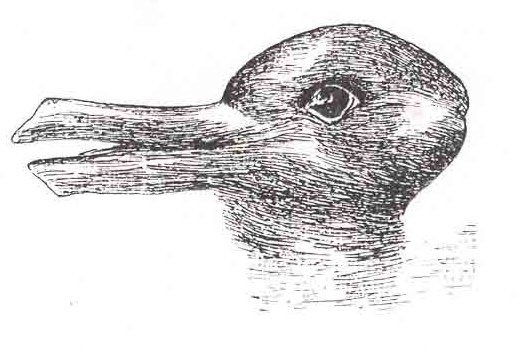
\includegraphics[width=.4\linewidth]{DuckRabbitIllusion}
\caption[Ambiguous Images]{An ambiguous image that could be either a rabbit or a duck. When participants were asked to identify the image initially, they could not provide an alternate interpretation of the figure later.}\label{fig:ambiguousrabbit}
\end{figure}

The ``software" of the visual system is of course more complex than the few modules listed here, but understanding attention, object perception, and how images are stored for later retrieval in the brain will make designing statistical graphics for the visual system easier and will also help with evaluating graphics based on the capabilities of the human visual system.

We have discussed the neural hardware of the visual system and some of the higher-level software that contributes to our ability to create and understand meaning in the world around us. Occasionally, our highly tuned perceptual system fails in unusual ways due to the heuristics and algorithms that were optimized for operation in a three-dimensional world where the main tasks were hunting, gathering, and avoiding predators. The next section will examine three interesting results of this tuning that are important to the design of statistical graphics as we transition from the psychophysics and cognitive psychology literature to statistics and human-computer interaction literature.

\subsection{Bugs and Peculiarities of the Visual System}\label{visualbugs}
\subsubsection{Logarithmic perception}\label{logarithmicperception} One of the earliest psychophysics researchers, Ernst Weber, discovered that the difference threshold, the smallest detectable difference between two sensory stimuli, increased proportionately with the magnitude of the stimulus. This statement, known now as Weber's Law, holds true for a large range of intensities of a number of senses. Numerically, Weber's Law is stated as
\begin{equation}\label{weberlaw}
\frac{\triangle S}{S} = K
\end{equation}
where $K$ is a constant called the Weber fraction, $S$ is the value of the standard stimulus, and $\triangle S$ is the difference between the standard stimulus and the test stimulus. So if a participant is given a 100-g weight and a 102-g weight and can just barely tell the difference between the two, then $K=0.02$ and we would assume that the the difference between a 200-g weight and a 204-g weight would be just barely detectable as well (Chapter 1, \citealt{goldstein}). While this example concerns the ability to distinguish weight, the same law holds for the ability to distinguish sounds of different intensities as well as intensity of colors. The tendency of the brain to perceive stimuli in a logarithmic fashion is true across many perceptual domains. In fact, when kindergarden children are asked to place numbers 1-10 along a number line, they place 3 in about the middle, just as one would expect from a logarithmic perspective. This ability disappears with mathematical education, but persists in those who are not given a formal education in mathematics, indicating that our brains are naturally wired to perceive numbers logarithmically \citep{varshney2013we}. Some sensory domains utilize logarithmic scales to measure stimuli; scales such as sound intensity, earthquake intensity, and frequency along the electromatic spectrum are logarithmic. Information theory suggests that logarithmic scaling provides optimal compression of information to minimize relative errors in perception while accounting for limits in our neural bandwidth. \citet{sun2012framework, varshney2013we} showed that a bayesian model for perception would result in a model that mimics the logarithmic relationship in Weber's Law. This suggests that the logarithmic nature of human perception is a result of an heuristic that increases processing power by reducing the neural bandwidth necessary to process information through quantization of continuous information and compression of discrete information. From a statistical graphics point of view, then, log-transformed scales should be used instead of linear scales for continuous color scales and for contour plots with a fixed number of contours, as this provides more information discrimination ability and mimics natural human perceptual tendencies. The reasons for this guideline are discussed more in section \ref{cognitiveload}.

\subsubsection{Colorblindness and color perception}\label{colorblindness}
Another common ``bug" in the visual system are mutations that change (or remove entirely) the cones in the retina. Such mutations are commonly termed ``colorblindness" and encompass many different types of mutations, shifts and deletions that affect color perception in the visual system. These mutations affect up to 5\% of the population, and are generally more common in males than they are in females, as two of the three genes producing cones are found on the X chromosome. Evolutionarily, these mutations are maladaptive for gathering plants (as finding red berries within green leaves is more difficult with the most common types of colorblindness), but may be adaptive for seeing camoflauged objects \citep{morgan1992dichromats}. In statistical graphics, however, these mutations often disrupt perception of standard color schemes used in maps, heatmaps, and divergent color scalings.
% Figure \ref{fig:USflag} shows the United States flag as seen by those with different types of color-blindness; the red and blue hues look radically different to those with different mutations.
%
% \begin{figure}[htbp]\centering
% 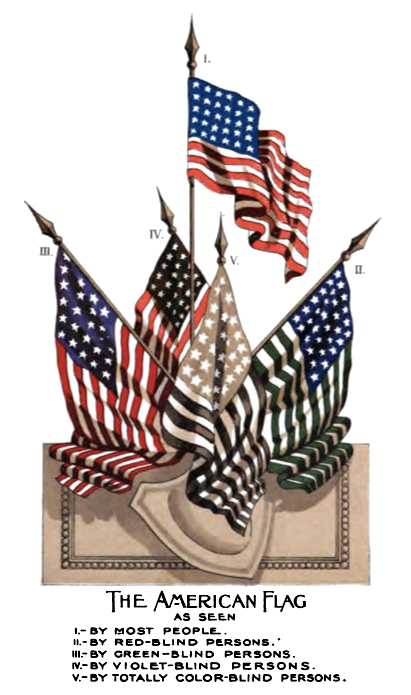
\includegraphics[width=.3\linewidth]{USflagColorBlind}
% \caption[Colorblindness and US Flags]{An 1895 illustration of the US flag as seen by those with different types of colorblindness.}\label{fig:USflag}
% \end{figure}
%

\begin{figure}[!htbp]\centering
\begin{minipage}[c]{.24\linewidth}
  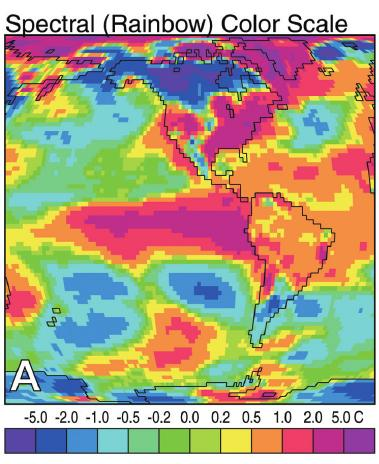
\includegraphics[width=\linewidth]{RainbowScaleOrig}
\end{minipage}
\begin{minipage}[c]{.75\linewidth}
\hfil\begin{subfigure}[b]{.32\linewidth}\centering
  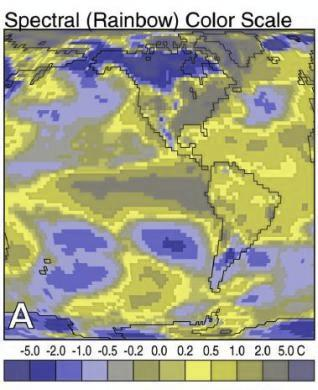
\includegraphics[width=\linewidth]{RainbowScaleOrig-protanopia}
  \caption{Protanopia}
\end{subfigure}
\hfil\begin{subfigure}[b]{.32\linewidth}\centering
  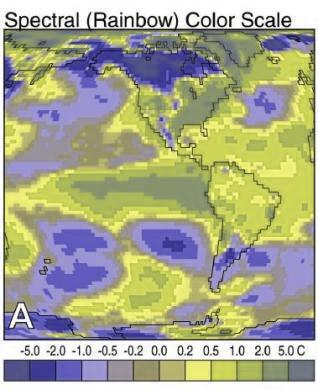
\includegraphics[width=\linewidth]{RainbowScaleOrig-deuteranopia}
  \caption{Deuteranopia}
\end{subfigure}\hfil
\begin{subfigure}[b]{.32\linewidth}\centering
  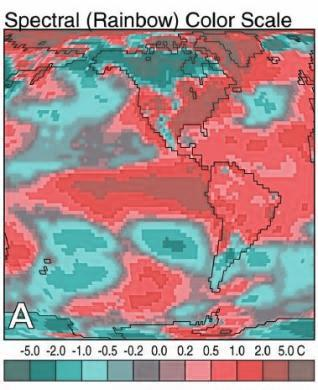
\includegraphics[width=\linewidth]{RainbowScaleOrig-tritanopia}
  \caption{Tritanopia}
\end{subfigure}

\hfil\begin{subfigure}[b]{.32\linewidth}\centering
  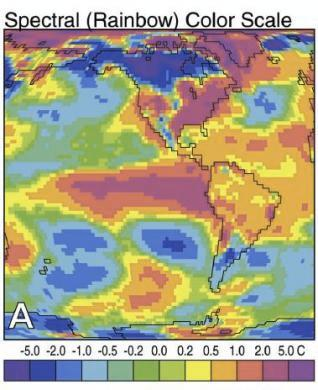
\includegraphics[width=\linewidth]{RainbowScaleOrig-protanomaly}
  \caption{Protanomaly}
\end{subfigure}\hfil
\begin{subfigure}[b]{.32\linewidth}\centering
  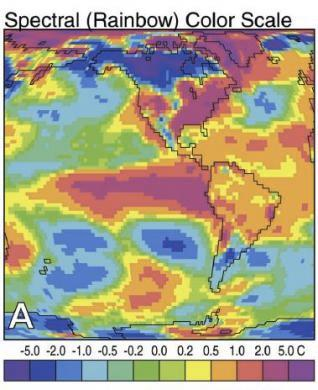
\includegraphics[width=\linewidth]{RainbowScaleOrig-deuteranomaly}
  \caption{Deuteranomaly}
\end{subfigure}\hfil
\begin{subfigure}[b]{.32\linewidth}\centering
  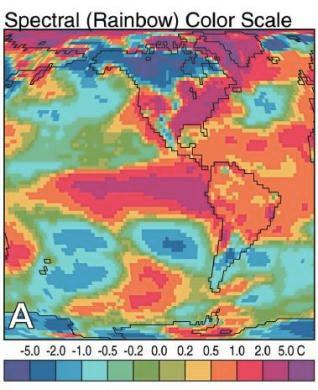
\includegraphics[width=\linewidth]{RainbowScaleOrig-tritanomaly}
  \caption{Tritanomaly}
\end{subfigure}\hfil
\end{minipage}

\caption[Colorblindness and Rainbow Color Schemes]{Rainbow color scheme with simulations of each of the six common types of color deficiency. The original image, on the left, is from \protect\citet{light2004end}. The top row of pictures on the right show simulations of the map when cones are entirely missing. The bottom row of pictures show simulations of the map when each cone is altered due to genetic mutation. }\label{fig:colorblindrainbow}
\end{figure}
% \comment{I can't tell a difference between the Protan* and Deuteran* pictures in figure \ref{fig:colorblindrainbow} at all. Is that just me?} % apparently not, normal color vision people seem to see it that way too.

In the natural world, many strategies can be used to compensate for colorblindness; the most common of these strategies is to look for textural variation instead of color variation (which may be why camoflauged objects are easier to see), but these strategies fail when viewing abstract, constructed visual stimuli, such as graphics, which may not have textural variation which corresponds to color variation. Compounding this problem, the rainbow color schemes that are commonly used are particularly vulnerable to misinterpretation by colorblind viewers. Figure \ref{fig:colorblindrainbow} shows a map using a rainbow color scheme (first shown in \citet{light2004end}) and simulated images showing what that map would look like to those with missing cones (-anopia) and cones with altered wavelengths (-anomaly). Simulations\footnote{provided by \url{http://www.color-blindness.com/coblis-color-blindness-simulator/}} show that rainbow color schemes are incredibly difficult for color-deficient individuals to read, because the opposite ends of the color spectrum appear extremely similar with mutations to the first or second cones. In addition, categorical rainbow color schemes require longer fixation times to identify regions of importance \citep{lewandowsky1993perception} and result in decreased recall accuracy compared to monochrome categorical color schemes. \citet{light2004end} provides color schemes that are more appropriate for those with color deficiencies, but not all of these schemes are appropriate for all types of color blindness. \citet{silva2011using} suggest many tools to recommend appropriate color schemes for colorblind users as well as tools to preview graphics as they might look to color-deficient or colorblind users.

Appropriately colored maps and graphs are not only useful for those who have impaired color vision, they can also be much easier to read for those with normal vision. \citet{rainbowcolor} suggest that color schemes which utilize the range of human color vision appropriately produce more aesthetically pleasing graphs and more accurately convey data in a form appropriate for the human perceptual system. Even some dual-color schemes may be problematic, as some evidence \citep{lewandowsky1993perception} suggests that these schemes are not infrequently inverted when encoded in memory, and are suboptimal for those with limited color perception as well as when printed in monochrome. Psychologically, color schemes which utilize both hue and intensity (for instance, transitioning from blue to red through white) require binding of two features, increasing encoding latency and the possibility of recall errors. Where possible, schemes utilizing only one feature (generally intensity, to preserve accessibility) are preferrable.

\subsubsection{Optical Illusions}
The ``software" programs presented in section \ref{Software} are generally efficient at completing everyday tasks: navigating the environment, avoiding predators (lions or cars, as the case may be), and identifying situations and objects relevant to the task at hand. These heuristic-style approaches produce suboptimal results when applied to more artificial tasks, such as reading statistical graphics. As a result, it is important to understand where conflicts between sensation and perception may occur, so that these conflicts can be dealt with or avoided entirely. In this section, we will discuss several optical illusions and explanations for their occurence based on the visual system.

\paragraph{Physiological Illusions} The illusions shown in figure \ref{fig:InhibitionIllusions} are illusions which occur due to the wiring of the brain. These illusions can generally be avoided in statistical graphics, but are difficult to counteract once they occur, as the illusion is literally hard-wired into the brain.

\paragraph{Gestalt Illusions} Some illusions occur due to a conflict of gestalt principles. Two of these illusions are shown in figure \ref{fig:GestaltIllusions}: the figure/ground illusion, and the illusory contour illusion.

\begin{figure}[htbp]\centering
\hfil
\begin{subfigure}[b]{.4\linewidth}\centering\vspace{.5cm}
  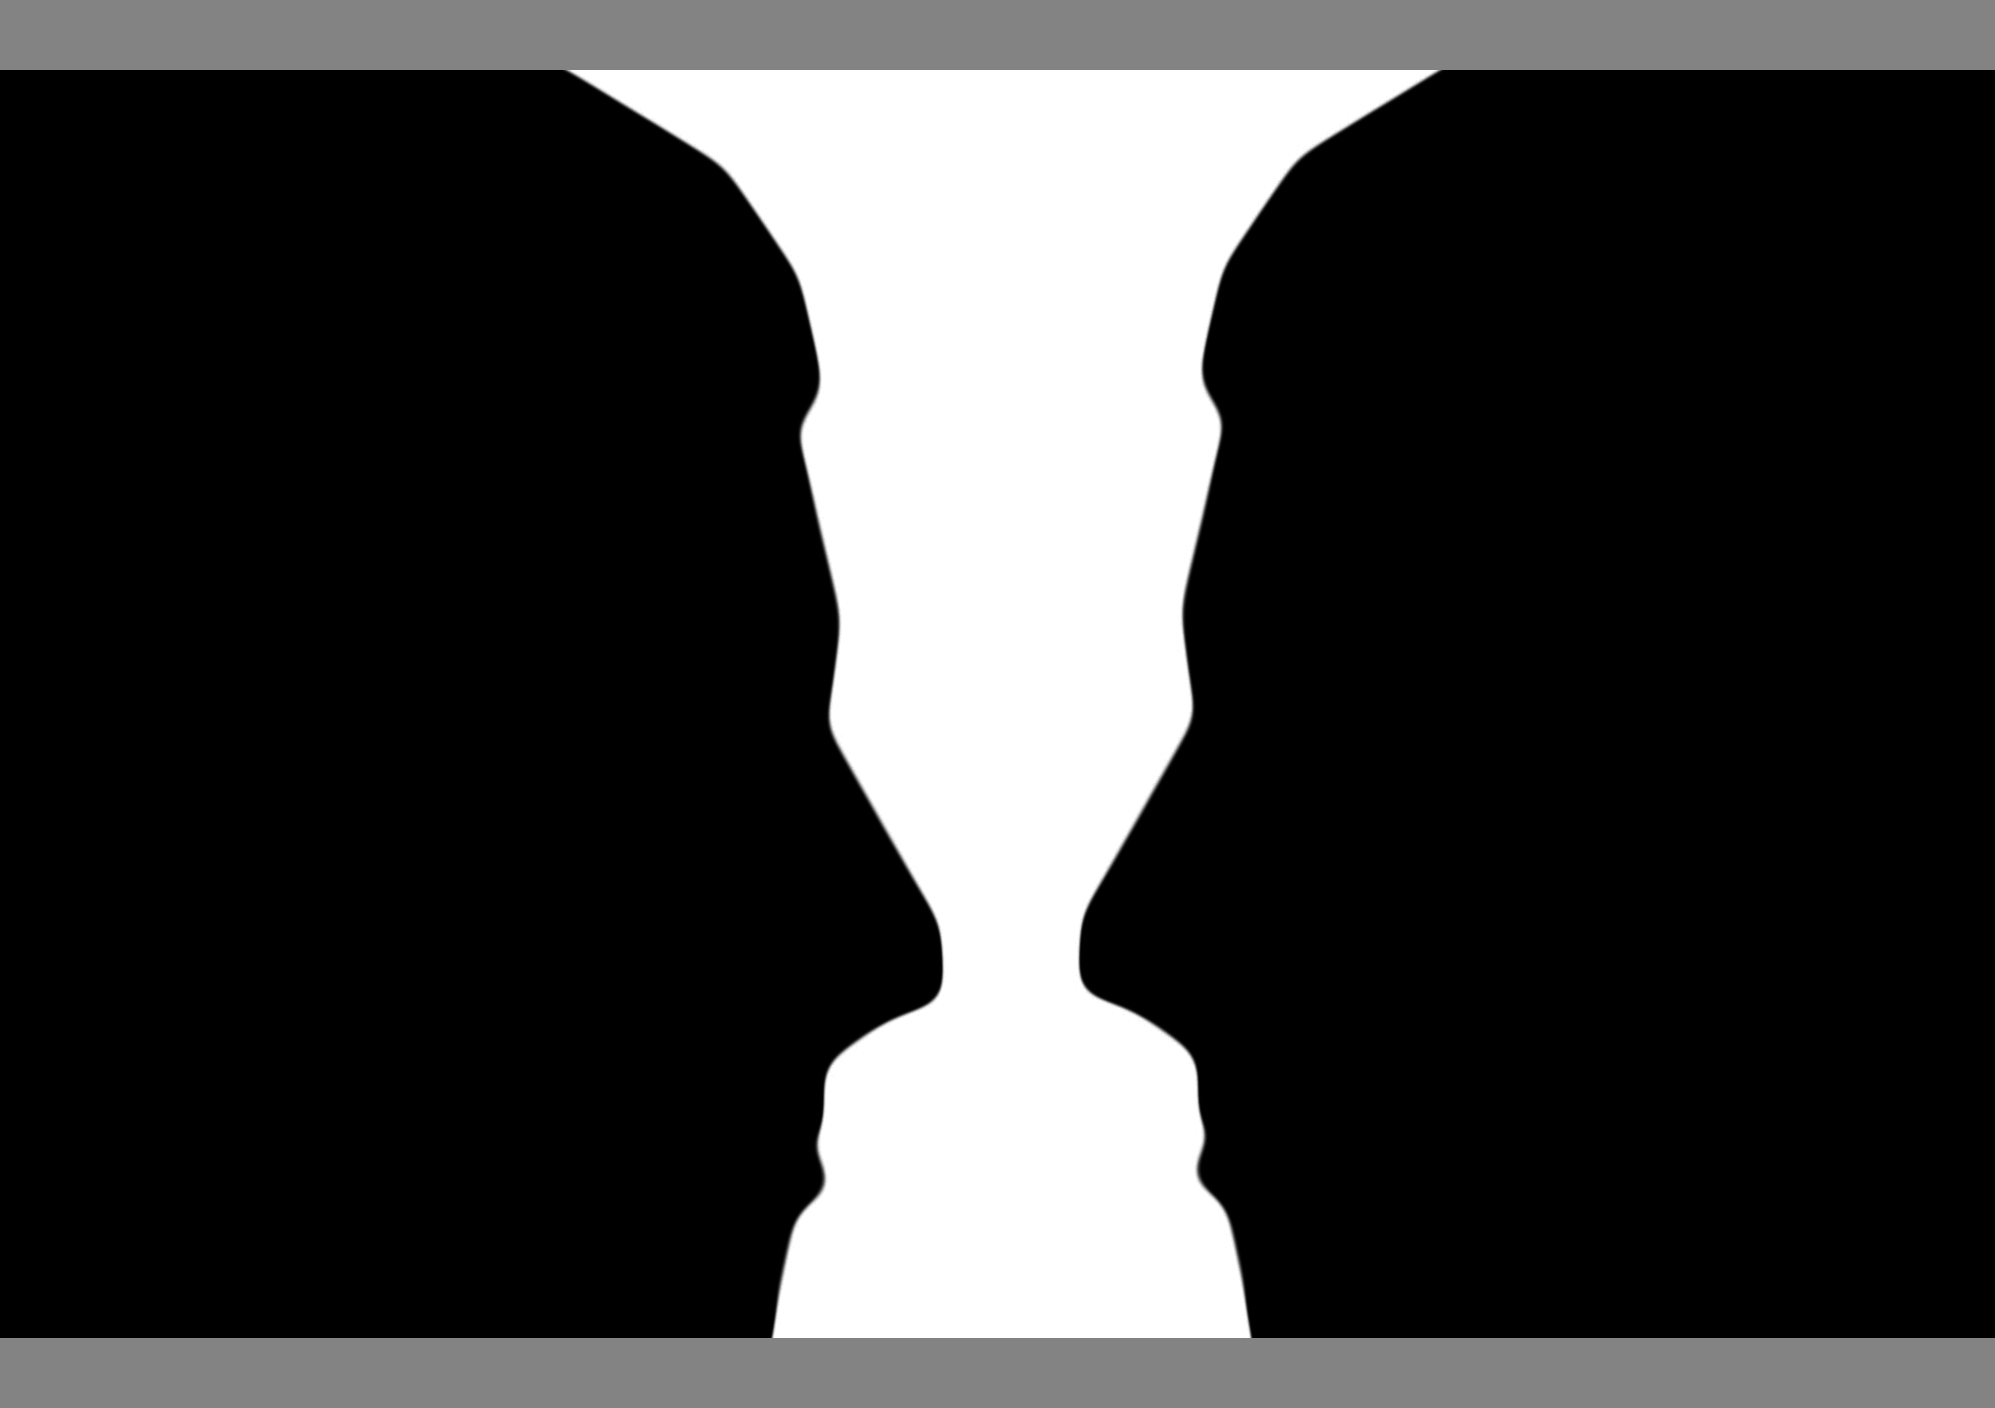
\includegraphics[width=\linewidth]{FigureVase}\vspace{1cm}
  \caption{Figure-Ground Illusion}
\end{subfigure}\hfill
\begin{subfigure}[b]{.4\linewidth}\centering
  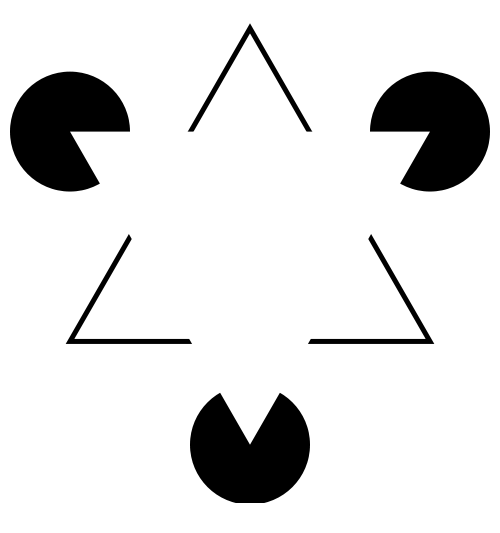
\includegraphics[width=\linewidth]{IllusoryContour}
  \caption{Kanizsa Triangle Illusion}
\end{subfigure}\hfil
\caption[Gestalt Illusions]{Illusions due to misapplied or ambiguous Gestalt rules.}\label{fig:GestaltIllusions}
\end{figure}

The figure/ground illusion depends on the color of the top and bottom edges of the picture; if the edges are black, the vase appears to be the central part of the image; if the edges are white, the faces appear to be the central part of the image. When the edges are omitted, the image seems to oscillate between a vase and the profile view of two heads. This is a result of ambiguity in identifying which part of the image is the background; when the top and bottom edges are present, that cue is sufficient to resolve the illusion. The Kanizsa triangle demonstrates the Gestalt principles of good form and continuity: We perceive objects that are partially obscured by a floating white triangle, even though no such triangle actually exists. The illusory triangle produces an image that is much simpler (3 circles, a black triangle outline, and a white triangle) than the objects that are actually displayed (3 partial circles and three V shapes arranged pointing in toward a central point). In addition to the existence of the illusory contour, we also perceive some depth to the image; that is, the white triangle is perceived as being above the other components of the image \citep{coren1983subjective}, as this is the only way to make sense of the set of stimuli in a simple fashion. In general, these gestalt principles make sense of the natural world, but when applied to artificial contexts, they occasionally produce unexpected results.

\paragraph{Depth illusions} Other optical illusions occur due to the optimization of the visual system for three-dimensional perception. These three-dimensional heuristics can produce unexpected or misleading results when applied to two dimensional objects.

\begin{figure}[htbp]\centering
\hfil
\begin{subfigure}[b]{.35\linewidth}\centering
  
\includegraphics[width=\linewidth]{PonzoIllusion}
  \caption{Ponzo Illusion}\label{fig:Ponzo}
\end{subfigure}\hfill
\begin{subfigure}[b]{.35\linewidth}\centering
  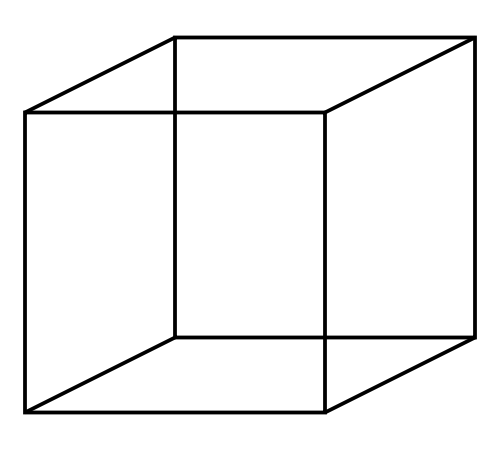
\includegraphics[width=\linewidth]{NeckerCube}
  \caption{Necker Cube}\label{fig:NeckerCube}
\end{subfigure}\hfil

\hfil
\begin{subfigure}[b]{.35\linewidth}\centering
  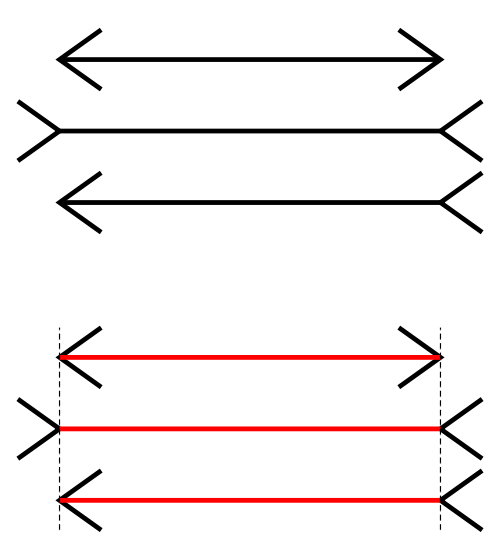
\includegraphics[width=\linewidth, angle=90]{MullerLyer}
  \caption{Muller-Lyer Illusion}\label{fig:MullerLyer}
\end{subfigure}\hfill
\begin{subfigure}[b]{.35\linewidth}\centering
  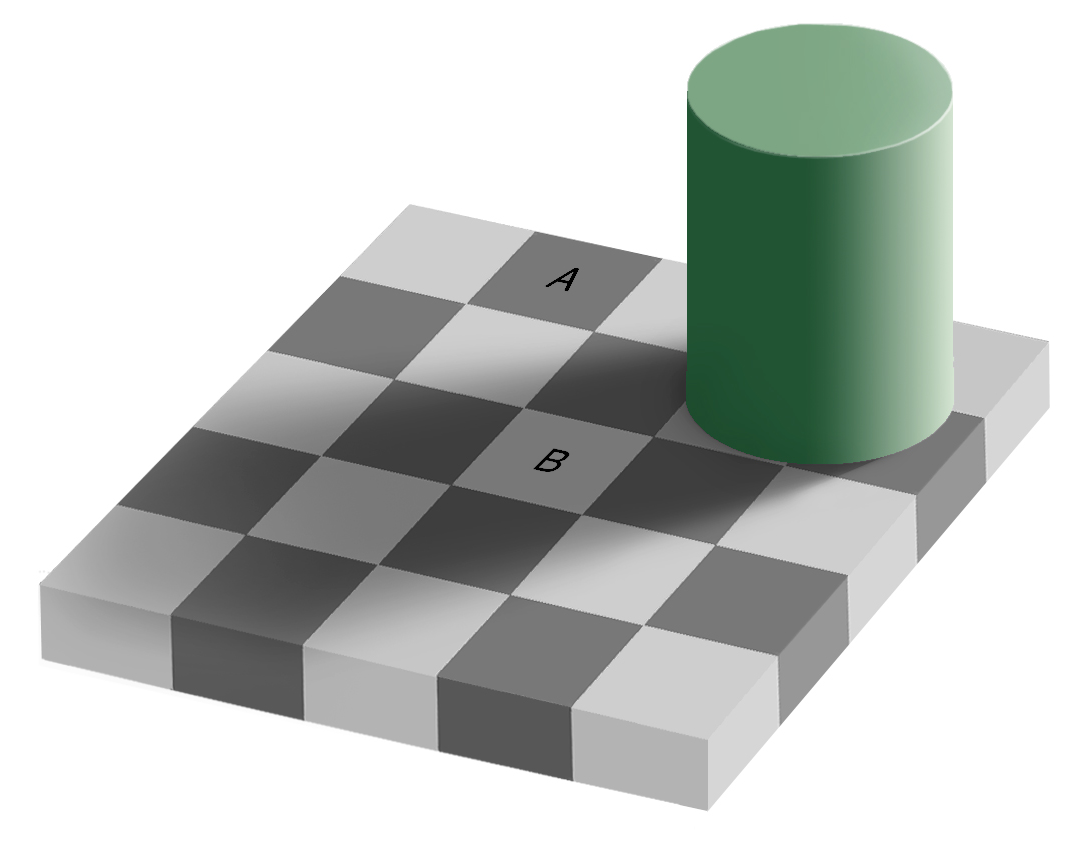
\includegraphics[width=\linewidth]{CheckerShadow}
  \caption{Color Constancy Illusion}\label{fig:ColorConstancy}
\end{subfigure}\hfil

\caption[Depth Illusions]{Illusions due to misapplied depth perception.}\label{fig:DepthIllusions}
\end{figure}
Figure \ref{fig:DepthIllusions} contains four of the more interesting optical illusions that result from ambiguous figures that trigger depth cues. The Ponzo illusion (figure \ref{fig:Ponzo}) suggests that the top line is longer than the bottom line, because of the implied convergence of the two vertical lines (to understand the natural scene that produces this illusion, consider railroad tracks converging at the horizon). The Necker Cube, shown in figure \ref{fig:NeckerCube}, can be seen such that the top-right face is closest to the viewer or alternately such that the bottom-left face is closest to the viewer. Due to the ambiguity in the image, it will often seem to ``flip" when the viewer temporarily loses focus on the image \citep{gregory1997knowledge}. The Muller-Lyer illusion (figure \ref{fig:MullerLyer}) is generally believed to result from misapplied depth cues as well - the left-most image would occur in nature as the exterior corner of a building, the middle image would occur when viewing an interior corner of the same building, further away from the viewer \citep{ward1977case, gregory1968perceptual, fisher1970experimental}. As a result of the illusion, the middle line appears to be longer than the first or third lines. Figure \ref{fig:mullerlyerhouse} shows the first two parts of the illusion in a context which removes the ambiguity through additional depth cues. The additional cues result in the resolution of the illusion. Finally, the color constancy illusion shown in figure \ref{fig:ColorConstancy} suggests that the square marked A is much darker than the square marked B, even though the two squares are the same color. This illusion results from our experiences with depth and shadows: square B is perceived to be the same color as the lighter-colored squares outside the shadow, while square A is perceived to be the same color as the other dark squares in the tile pattern, regardless of the actual color due to the shadow.

\begin{figure}[htbp]\centering
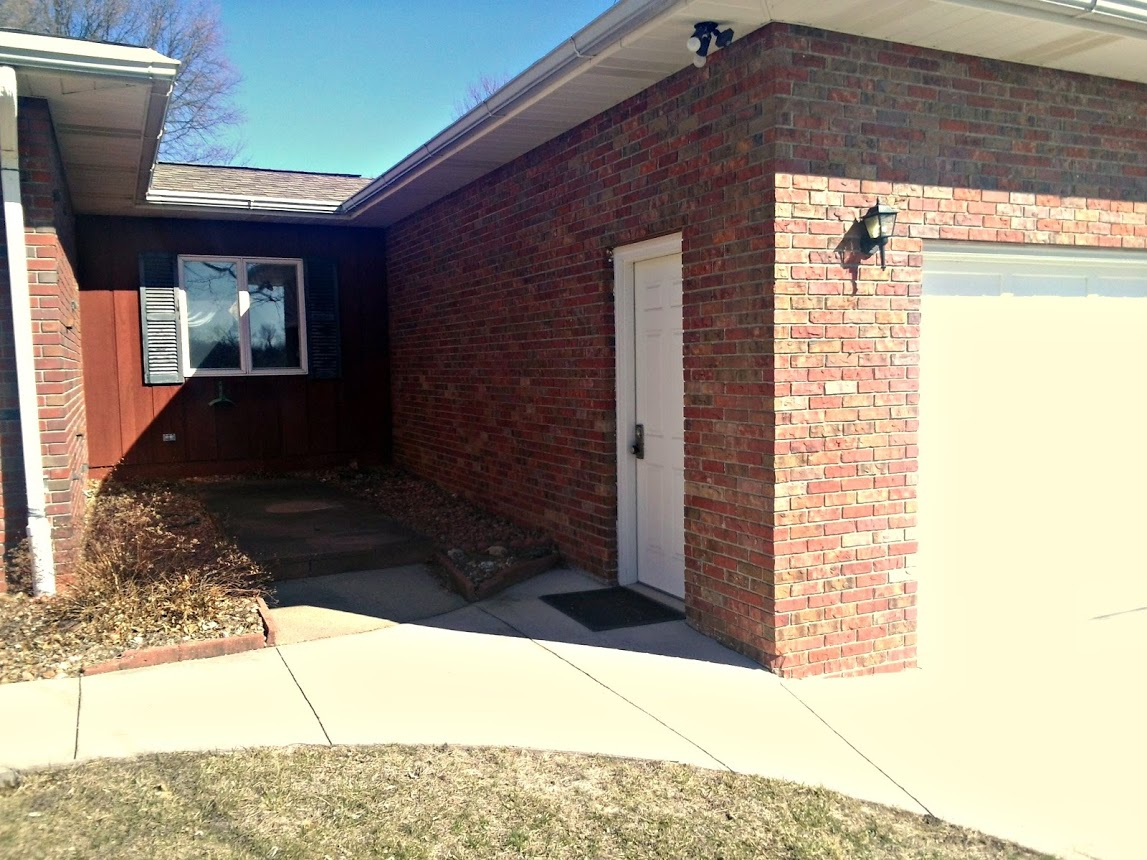
\includegraphics[width=.5\linewidth]{mullerlyerhouse}
\caption[Muller Lyer Real World Context]{The Muller-Lyer illusion in a non-ambiguous three-dimensional context.}\label{fig:mullerlyerhouse}
\end{figure}

Depth illusions in particular result from a conflict between our experience with the three-dimensional world and the appearance of two-dimensional ambiguous stimuli. The Necker cube ``flips" because there are two physical objects that could produce the same retinal image, the Muller-Lyer illusion exists because our experience with the three-dimensional world is harnessed inappropriately for a two-dimensional figure, and the color-constancy illusion exists because our brains automatically correct a pseudo three-dimensional image to represent the reality of that image in the real world. These conflicts occur in statistical graphics as well: certain graphical configurations can trigger a three-dimensional heuristic in the brain and lead to misleading conclusions \citep{sineillusionjcgs,parallelsets}.

\todo[inline]{Add more information on Sine Illusion and other illusions?}

There are other optical illusions that have the potential to appear in statistical graphics but are not easily classified (or necessarily easily explained). Two of these illusions are considered below.
\paragraph{Other Important Optical Illusions}
Certain illusions do not lend themselves to simple classification. While many illusions are the result of multiple concurrent processes in the brain, these illusions may not even be fully understood. The Poggendorff illusion, shown in figure \ref{fig:poggendorff}, is one such illusion.

\begin{figure}[htbp]\centering
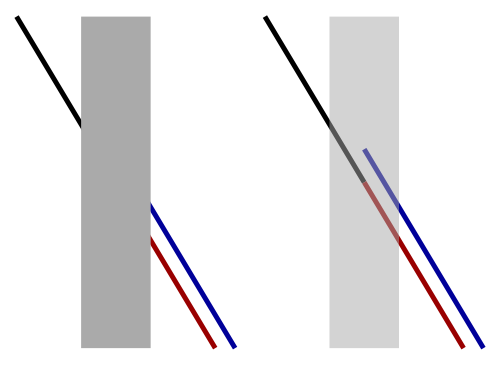
\includegraphics[width=.4\linewidth]{Poggendorff}
\caption[The Poggendorff Illusion]{The Poggendorff Illusion. The left figure shows a black line which is obscured by a grey rectangle; it appears that the blue line would intersect the black line if the rectangle were not present. In fact, the black line and the red line are co-linear, and the blue line is parallel to both other lines.}\label{fig:poggendorff}
\end{figure}

\citet{gregory1963distortion, gregory1997knowledge} suggests the Poggendorff illusion is similar to the Muller-Lyer illusion in that it results from misapplied depth cues, but \citet{green1963poggendorff, ward1977case} found no evidence that participants viewed this illusion in any three-dimensional context. Instead, \citet{green1963poggendorff} suggests that the illusion results from a tendency to perceive acute angles as less acute and obtuse angles as less obtuse than the image suggests. As the illusion disappears as the angle of the line segment approaches horizontal, this seems to be a reasonable explanation, but it is almost certainly not complete \citep{morgan1999poggendorff}, as the illusion survives in forms which do not preserve the acute angle intersections. Regardless, this illusion can make it difficult to read line graphs \citep{amer2005bias, poulton1985geometric} if proper precautions (use of reference lines and grid lines) are not taken.

The second of these illusions is the cafe wall illusion, shown in figure \ref{fig:cafewall}, named because this tile pattern is apparently common in cafes.


\begin{figure}[htbp]\centering
\hfil
\begin{subfigure}[b]{.4\linewidth}\centering
  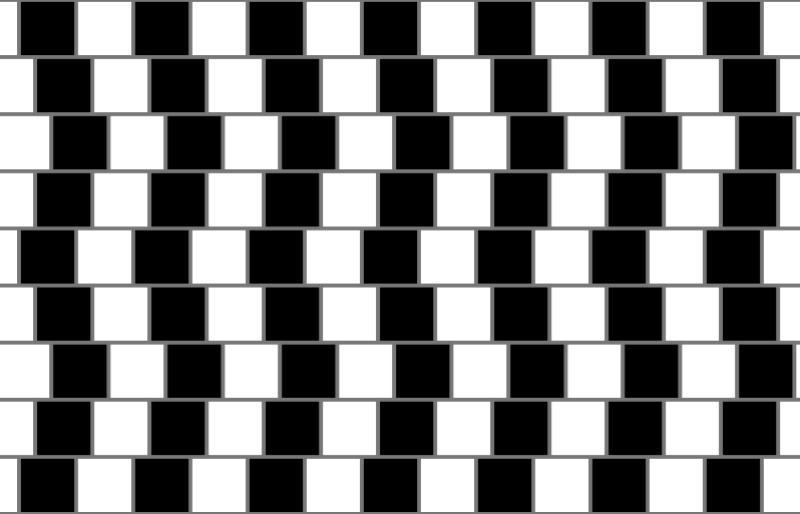
\includegraphics[width=\linewidth]{CafeWall}
  \caption{Original Cafe Wall Illusion}\label{fig:CafeWallOrig}
\end{subfigure}\hfil
\begin{subfigure}[b]{.4\linewidth}\centering
\begin{knitrout}
\definecolor{shadecolor}{rgb}{0.969, 0.969, 0.969}\color{fgcolor}

{\centering 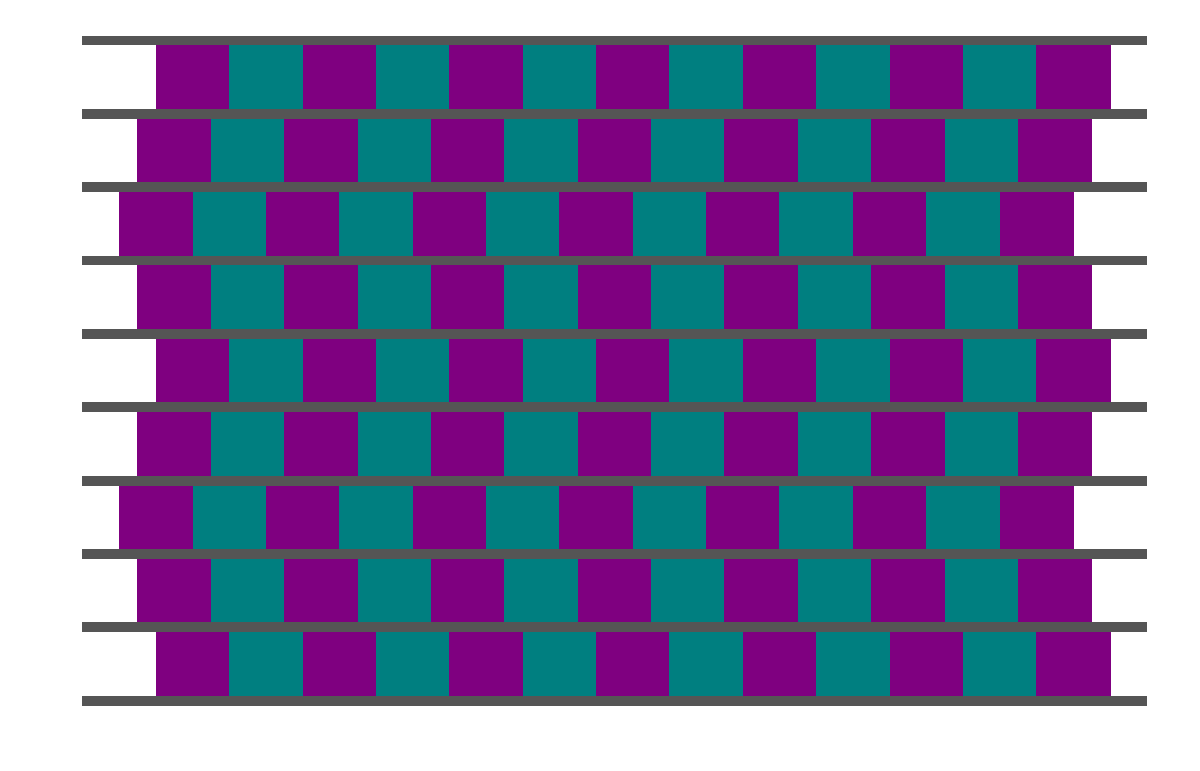
\includegraphics[width=\linewidth]{Figure/fig-cafewall-1} 

}



\end{knitrout}
  \caption{Isoluminant Cafe Wall Illusion}\label{fig:CafeWallIso}
\end{subfigure}\hfil
\caption[Cafe Wall Illusion]{The Cafe Wall illusion. The lines between rows of black and white tiles are parallel but appear to be tilted. The second image shows the isoluminant version, which mitigates some of the illusion but does not entirely eliminate the effect.}\label{fig:cafewall}
\end{figure}

The cafe wall illusion is in part due to the contrast between light and dark zones (as in the mach bands and hermann grid illusion), and much of the illusion is resolved when the black and white tiles are replaced with isoluminant colors, but some of the illusion still remains. \citet{westheimer2007irradiation} suggests that this portion of the illusion is because the position of a black-white border will be biased to appear closer to the black side of its physical location, an effect which is compounded in the cafe wall illusion to produce the appearance of tilted lines. This illusion, while not explicitly found in most statistical graphics, shows that even simple (and pleasant) configurations of geometric objects can wreak havoc in the brain under the right circumstances. In fact, the illusion is so simple that it is also known as the ``Kindergarten illusion", but its cause is sufficiently complex that it has not been fully explained by psychologists or neuroscientists.

\subsection{Cognitive Load}\label{cognitiveload}
It is fairly well established that statistical graphics are useful in part because they can replace long tables of data, summarizing information in a form that is much easier to understand and mentally maniuplate; as such, it would not be out of line to suggest that graphics require less cognitive load than tables of the same data. When we discuss cognitive load, we typically mean the limits in short-term memory, cognitive manipulation, attention, and mental bandwidth that bound our ability to take in new information and draw conclusions from that information. In this section, we will briefly discuss some of these considerations.

\paragraph{Short Term Memory} A famous paper in memory and cognition \citep{miller1956magical} suggests that active memory can contain only 7 (plus or minus two) chunks of information. A chunk of information could be a single letter or number, a meaningful collection of several letters or numbers (e.g. a word or an area code), or an association. This limitation is important in designing information for graphical consumption. For instance,  the number of categories in legends should be limited to 7, to allow a viewer to store the associations within the legend and then use that information to understand the graph. Abuse of this limitation is referred to as a ``color mapping attack" in \citet{conti2005attacking}, a paper detailing the various ways to ``attack" a human visualization system. Similarly, viewers should not be expected to remember more than 7 ``chunks" of information from a single graph. Due to these limitations in memory, when a single color scale is used to represent more than one order of magnitude of variation, using a logarithmic scale provides more optimal information scaling than using a linear color scale \citep{sun2012framework, varshney2013we}.

\paragraph{Information Integration}
Integrating multiple dimensions of information (or mentally combining multiple graphics) is another area which can strain the ability of the brain to utilize information effectively. Well-constructed graphs can help the brain to integrate information by connecting points across dimensions (through the use of regression lines, clustering, etc.), which creates ``chunks" of information that can then be stored in memory in a more compressed format. These chunks are useful because they allow people to draw conclusions from multiple sets of data across multiple dimensions \citep{gattis1996mapping}. Poorly created graphics may make this task harder or even promote the encoding of misleading chunks; for instance, data that is overplotted may obscure the important trend and may also produce chunks which lead to the wrong associations being stored in memory. This integration limitation is very much related to short-term memory, but is also constrained by mental effort limitations and processing capacity. As a result, it is important to reduce the effort required to integrate multiple graphics.

\paragraph{Attention}
Human attention is limited; thus visualizations which do not focus attention on important aspects of the data are likely to confuse the reader. \citet{eda} said ``The greatest value of a picture is when it forces us to notice what we never expected to see". When there are too many salient features to notice anything in particular, attention is split too many ways to gain useful information from the picture. Graphics should present data in a controlled fashion, so that focused attention is rewarded with useful information taken from the graph. \citet{conti2005attacking} describes graphs that do not follow this principle as ``processing attacks", in that the overload the ``CPU" with needless calculations and mental manipulations that are ultimately futile to understanding the data.

The consequence of the limits of human perception and processing capacity is that there is a limited amount of information one can expect to portray graphically; thus graphics should be designed to most efficiently communicate information so that this cognitive overload does not occur. The next section presents studies which examine the perception of graphs and charts directly across a wide range of perceptual levels and experimental conditions.

\section{Statistical Graphics}
Psychologists who study graphical perception are generally concerned with the underlying mechanisms of effects within the brain, and thus study very simple graphics and lower-level perceptual effects. In statistics, the literature is somewhat more variable; \citet{cleveland:1985} produced the seminal paper on the subject, but outside of that work, there are relatively few papers that examine the accuracy of judgments made from graphs through user studies that mimic the way graphs are used in practice. There have been a few papers in other disciplines; business and communications researchers occasionally study graphs and charts as well. As a result, the literature in this area is scattered across many disciplines. In order to organize this section effectively, we will begin with the lower-level graphical perception literature and conclude with studies that have more external validity and are applicable to statistical practice. For the purposes of the following sections, lower-level perception research is research which involves either extremely simple graphical elements (or non-graphical research which applies directly to graph perception processes), or which does not require attention (pre-attentive features of graphics). These experiments provide some information, but are less informative than experiments which utilize more complex graphics in realistic scenarios.

\subsection{Preattentive Perception of Statistical Graphics}\label{LowLevelGraphics}
Much of the lower-level research within the statistical graphics literature has been performed by those within the psychological community that study human information processing. In particular, \citet{healey1999large, healey2012attention} have produced several papers studying the accuracy of conclusions viewers can make after less than 1/2 of a second of viewing an image. As discussed in section \ref{AttentionPerception} and demonstrated in figure \ref{fig:preattentive}, certain features do not require individual focus to process; these features are called \emph{preattentive} and can be detected on the first glance (typically within 250ms). Healey's work focuses on determining which features can be detected in a pre-attentive fashion, and whether a hierarchy of features exists when these features are combined. Healey suggests that for three-dimensional displays, the 3d layout is determined first, surface structure and volume are determined next, followed by object movement (if present), luminance gradients, and color; he suggests that if there are conflicts between these 5 levels, priority is given to an earlier process \citep{healey2012attention}. \citet{healey1999large} showed that if visualizations are carefully constructed to conform to the architecture of the human visual system (isoluminant colors, removing certain background patterns from textural arrays), visual estimation tasks can be performed preattentively. The experiment also revealed an interference effect between texture and color that corresponds to previously documented interference between preattentive features \citep{treisman1985preattentive}. Figure \ref{fig:preattentiveinterference} demonstrates the interference effect; it is much easier to locate the target point in figure \ref{fig:preattentiveshape} or figure \ref{fig:preattentivecolor} than it is to locate the target in figure \ref{fig:preattentiveinterference}.





\begin{figure}[htbp]\centering
\begin{subfigure}[b]{.3\linewidth}\centering
\begin{knitrout}
\definecolor{shadecolor}{rgb}{0.969, 0.969, 0.969}\color{fgcolor}

{\centering 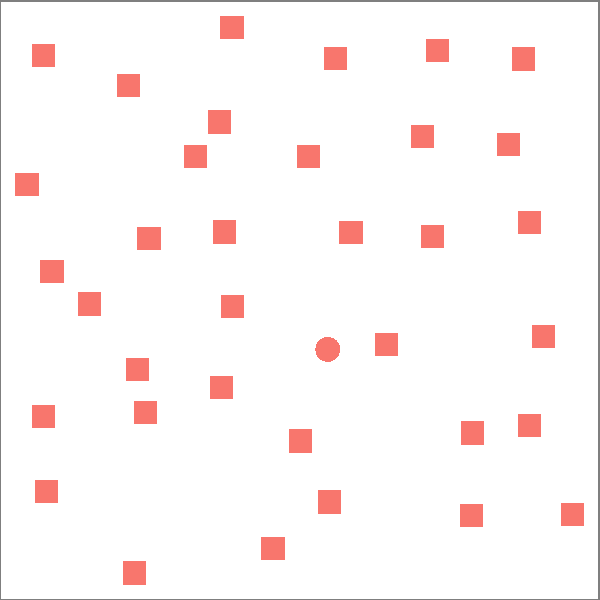
\includegraphics[width=\linewidth]{Figure/fig-preattentive1-1} 
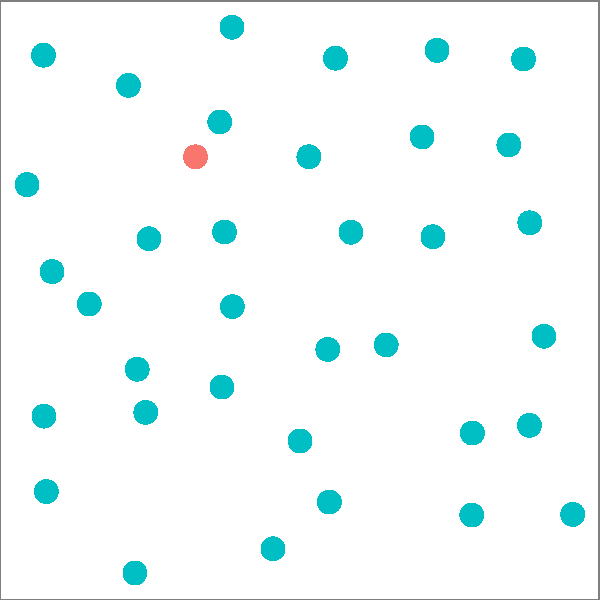
\includegraphics[width=\linewidth]{Figure/fig-preattentive1-2} 

}



\end{knitrout}
  \caption{Shape}\label{fig:preattentiveshape}
\end{subfigure}\hfill
\begin{subfigure}[b]{.3\linewidth}\centering
\begin{knitrout}
\definecolor{shadecolor}{rgb}{0.969, 0.969, 0.969}\color{fgcolor}

{\centering 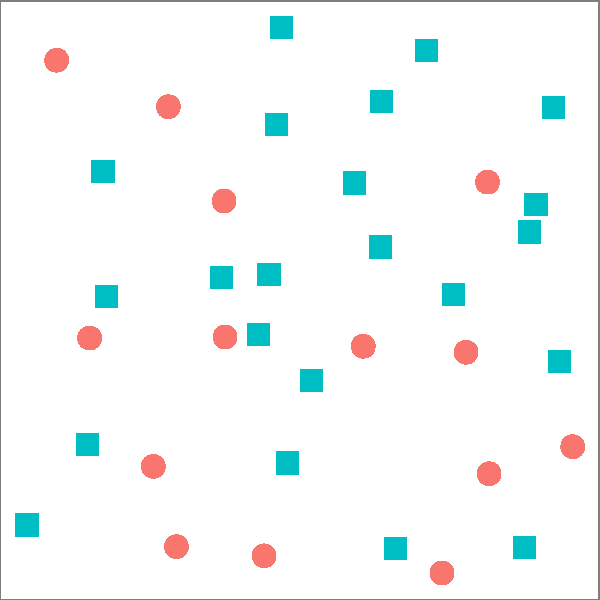
\includegraphics[width=\linewidth]{Figure/fig-preattentive2-1} 

}



\end{knitrout}
  \caption{Color}\label{fig:preattentivecolor}
\end{subfigure}\hfill
\begin{subfigure}[b]{.3\linewidth}\centering
\begin{knitrout}
\definecolor{shadecolor}{rgb}{0.969, 0.969, 0.969}\color{fgcolor}

{\centering 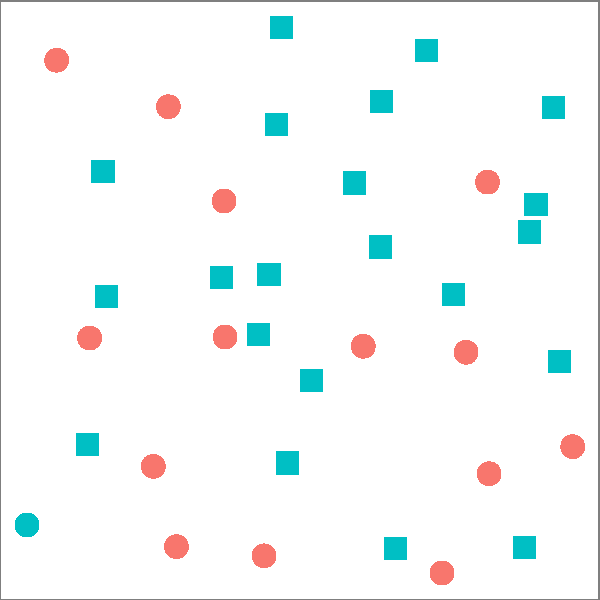
\includegraphics[width=\linewidth]{Figure/fig-preattentive3-1} 

}



\end{knitrout}
  \caption{Interference}\label{fig:preattentiveinterference}
\end{subfigure}
\caption[Preattentive Features and Interference]{Shape and color are detected preattentively in figures (a) and (b), but interfere in figure (c) so that location of the target in (c) is no longer preattentive.}\label{fig:preattentive}
\end{figure}

Healey's work on preattentive perception is interesting, and provides a reasonable approach to creating graphics compatible with the human visual system, but his work is largely focused on multidimensional displays and his focus on preattentive processes limits the applicability of his work to statistical graphics. In particular, most graphics are created with the idea that a viewer will spend more than one second looking at the graph, so not all features need to be preattentive to be useful. In addition, many of the multidimensional displays he designs are very load-intensive to understand; with so many additional dimensions, the viewer must spend considerable time understanding the scales and legends which correspond to each variable (feature integration over multiple dimensions is time intensive and generally not preattentive). In the next section, we will examine the literature concerning higher-level graphical perception, including perception at the attentive level and which types of graphs are more accurately perceived by viewers.

% \todo[inline]{Add section examining psychological literature (treisman) for lower-level measurement accuracy style studies?}

\subsection{Conscious Perception of Statistical Graphics}\label{HighLevelGraphics}
Graph perception from a statistician's point of view is more focused on the attentive stage of perception: When asked to answer a question using a graph, what parts of the graph are useful, and how is the information transferred from the image to working memory in the brain? Several models have been proposed to describe this process; of these, the set of ``task models" and ``integration models" seem to be most consistent with empirical evidence.

\subsubsection{Models of Graph Perception}
These task-based models suggest that task-based graphical perception, e.g. using a graph to answer a specific question involves several stages of information processing \citep{ratwani2008thinking}.
\begin{enumerate}
\item Parts of the question are read several times
\item The graph is searched for relevant information, with focus shifting from the graph axes to the main part of the graph and back again (pattern recognition)
\item Once information is found, the focus shifts between the important part of the graph and the legend several times in order to keep the relevant information in working memory (conceptual relations produce quantitative meaning from visual features)
\item The question is answered and the participant moves on to another task (the question is related to the encoded quantitative features)
\end{enumerate}

These steps are illustrated in figure \ref{fig:taskgraph}.


\begin{figure}[htbp]
\textbf{Question:} What is the relationship between the length of the eruption and the time between eruptions for Old Faithful?
\begin{center}
\begin{minipage}[c]{.45\linewidth}
\begin{knitrout}
\definecolor{shadecolor}{rgb}{0.969, 0.969, 0.969}\color{fgcolor}

{\centering 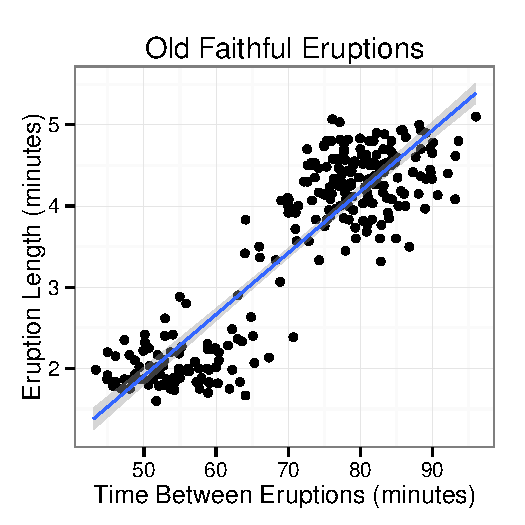
\includegraphics[width=\linewidth]{Figure/fig-steps-1} 

}



\end{knitrout}
\end{minipage}
\begin{minipage}[c]{.54\linewidth}
\textbf{Sample mental steps: }
{\small
\begin{enumerate}
\item Understand the question, identify ``length of eruption" and ``time between eruptions" as things to search for in the graph.
\item Look for ``length of eruption" on the axes, determine that the $y$ coordinate contains that information. Look for ``time between eruptions" on the axes and determine that the $x$ coordinate contains that information. Verify that these quantities are indeed what is being sought by re-reading the question.
\item Establish that as the time between eruptions increases, the length of the eruption increases. Note that there seems to be a bimodal distribution of points.
\item Answer the question: As the time between eruptions increases, the length of the eruption seems to increase.
\end{enumerate}
}
\end{minipage}
\end{center}
\caption[Task analysis of a simple graph]{Task analysis of a simple graph-based task. The graph shows the length of the eruption of Old Faithful as a function of the waiting time between eruptions, with a corresponding sample ``mental dialog" of the perceptual tasks involved in answering the question in response to the graph, according to \protect\citet{shah2005cambridge}. }\label{fig:taskgraph}
\end{figure}

Working within this task-oriented framework, researchers have explored the ``search" portion of the task-based model, the information integration portion of the model, and the types of graphs which facilitate both the ``search" and ``integration" portions of the task. Integration models modify the above sequence to allow for more complex graphical relationships to be assimilated, such that a viewer cycles between stages (2) and (3) several times in order to encode different portions of the graph. The time required for each of these steps may also change in accordance with the reader's familiarity with the task and graphic style; those who are more familiar with similar graphics may be able to encode information faster and in larger chunks and thus answer the question more quickly \citep{carpenter1998model}.



\begin{figure}[htbp]\centering
\begin{subfigure}[b]{.45\linewidth}\centering
\begin{knitrout}
\definecolor{shadecolor}{rgb}{0.969, 0.969, 0.969}\color{fgcolor}

{\centering 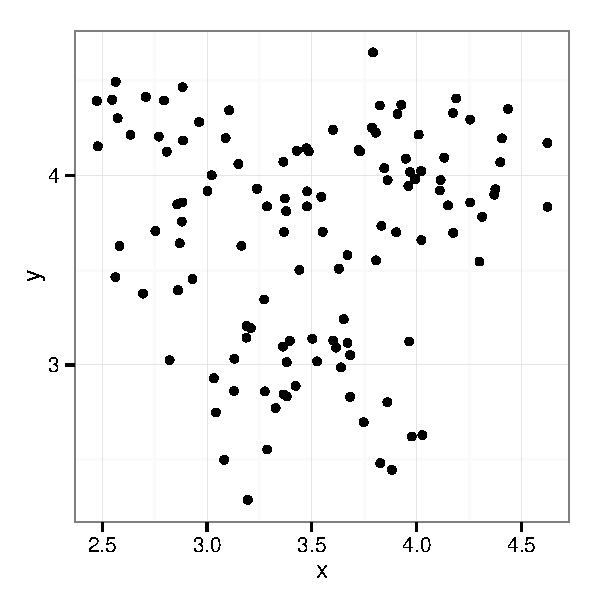
\includegraphics[width=\linewidth]{Figure/fig-clustering-a-1} 

}



\end{knitrout}
  \caption{Proximity-based grouping}
\end{subfigure}\hfill
\begin{subfigure}[b]{.45\linewidth}\centering
\begin{knitrout}
\definecolor{shadecolor}{rgb}{0.969, 0.969, 0.969}\color{fgcolor}

{\centering 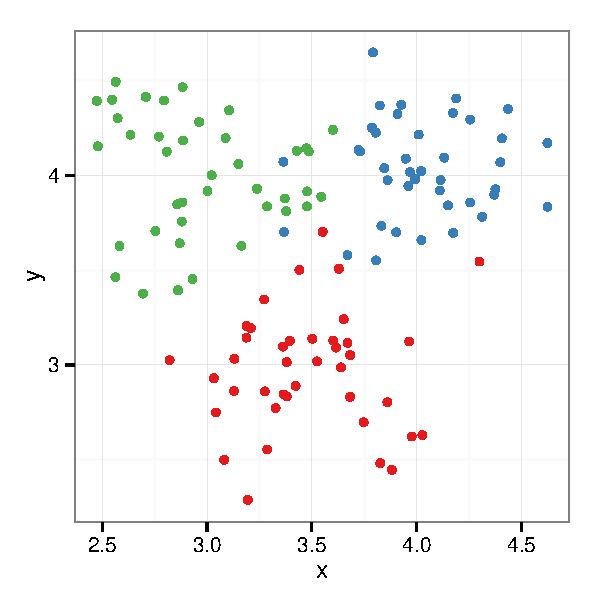
\includegraphics[width=\linewidth]{Figure/fig-clustering-b-1} 

}



\end{knitrout}
  \caption{Proximity and Similarity-based grouping}
\end{subfigure}\hfill
\caption[Chunking in Graphs]{The utility of chunking in graph perception. Graph (a) could potentially be described as three distinct clusters of points rather than 120 individual points, but it is much easier to draw conclusions from graph (b), which has colored points that clearly show the grouping structure in the data. The second figure would more probably be encoded and described as three groups of 40 points, which serves as a form of mental data compression.}\label{fig:clustering}
\end{figure}

Analyzing graphs using task-based models emphasizes the importance of spatial relationships between graphical elements. The gestalt laws of proximity and similarity dictate that items which are close together or physically similar (the same shape or color) are perceived as a group; this spatial perception creates ``chunks" of the graph which may be encoded as single objects and thus reduce the mental bandwidth necessary to process the image. Figure \ref{fig:clustering} shows the advantage of ``chunks" in graphs, as the second graph shown is much easier to describe and understand than the first graph, even without the contextual meanings of the variables. Of graphics that present information of similar complexity, graphics that require less effort to understand and search for relevant information are preferrable \citep{cleveland:1985}. More complex models of the graphical perception process suggest that data are integrated on a visual level and then further integrated on a cognitive level, to form successive clusters of information. Once these clusters are formed, further information can be integrated by comparing and contrasting different clusters to understand the higher-level meaning in the graph \citep{ratwani2008thinking}. Graph types which cater to this hierarchical clustering mechanism may be more easily understood by viewers than graphs that do not provide information in a manner easily assimilated by the human brain. Based on this information, facets of graphs may be particularly useful for mapping multidimensional data to provide ``chunks" of information in a relevant manner that can be integrated into the viewer's working conceptual understanding of the dataset. Additionally, color schemes and appropriate labeling of graph features which reduce the amount of work necessary to integrate numerical information from a legend into the visual representation of the graph facilitate graphical inference \citep{carpenter1998model}.

From a statistical perspective, much of the literature involved in understanding graph perception from a task-analysis point of view focuses on simple graphics, such as side-by-side bar graphs or line graphs, and straightforward tasks of reading information from the graph accurately, rather than examining model assumptions or making inference beyond the data. The psychologocial mechanisms involved in processing simple graphics are perceptual, and typically require direct comparisons rather than mental manipulation in order to satisfy the tasks posed by the researchers \citep{trickett2006toward}. More complicated graphics and more sophisticated tasks may require comparison of two or more distinct graphs and may utilize working memory and spatial reasoning; these situations are not as well studied \citep{shah2005cambridge}. We begin first with the simple tasks of graph comprehension, and will summarize work with more complicated graphics at the end of this section.

\subsubsection{Perception of Simple Graphs}
A series of experiments by \citet{cleveland:1984, cleveland:1985} studied basic perceptual tasks in graphical perception to produce a relative ordering of graphical elements by the accuracy of participant conclusions. This ranking is shown in Table \ref{clevelandranking}. Other researchers \citep{kosslyn1994} have collapsed this ranking into position/length/angle and area/volume, as the difference in accuracy between categories 1, 2, and 3 is small compared to categories 4 and 5.
\begin{table}[htbp]\centering
\begin{tabular}{ll}
\hline
Rank & Task\\\hline
1 & Position (common scale)\\
2 & Position (non-aligned scale)\\
3 & Length, Direction, Angle, Slope\\
4 & Area \\
5 & Volume, Density, Curvature\\
6 & Shading, Color Saturation, Color Hue\\\hline
\end{tabular}
\caption[Cleveland \& McGill's ordering of graphical tasks]{\protect\citet{cleveland:1984, cleveland:1985} ordering of graphical tasks by accuracy (adapted from both papers and \protect\citealt{shah2005cambridge}). Higher-ranking tasks are easier for viewers than low-ranking tasks and should be preferred in graphical design.}\label{clevelandranking}
\end{table}

The particular task required of participants in experiments also has an effect; \citet{simkin1987information} found that readers were more accurate in determining position when presented with a bar graph, but when readers were presented with a pie chart, they were more accurate at determining proportional judgments (using angles). This finding contradicts \citet{cleveland:1984} to some degree and suggests that the experimental design and specific task are important in evaluating these sorts of user studies; the contradictory results also suggest that graph type is an important influence in determining what information viewers encode from the graph. This conflict also illustrates that the user's attention and past experience influence the judgments they make from a given graph: when participants were asked to provide a summary of the graphic, their answers depended on the type of display: bar charts elicited a comparison judgment, pie charts elicited proportional judgments \citep{simkin1987information}. Similarly, when presented with a line graph, viewers are more likely to summarize the graph in terms of the slope of the trend line (even when the x-axis is discrete); when presented with a bar graph, viewers summarize the information using discrete comparisons \citep{carswell1987information, shah2005cambridge}. The task and the graph format interact to influence viewer perceptions, thus, when creating graphics, statisticians should match appropriate graphical formats to meaningful conclusions about the data.

The task requirements are mediated by the limits of human processing ability. Chernoff faces, once proposed for visualizing multidimensional data, are difficult to read because viewers are unable to store the legend and the image in working memory; comparisons must be made serially and with conscious attention \citep{shah2005cambridge}, and data features may not map well to relatable facial features \citep{lewandowsky1989perception}. Similarly, while color does not generally correspond to precise quantitative information, certain color schemes utilizing hue, saturation, and brightness together can provide an implicit numerical ordering that does not place exceptional demands on working memory \citep{shah2005cambridge}. Color schemes which correspond to everyday situations (e.g. using a blue to red scale for low to high temperatures) may also reduce the demand on working memory (though such a scale may be problematic due to principles of color perception). While specific numerical judgments would still require selective attention, the ``gist" of a graph using such schemes may be understood fairly quickly.

It is important to consider working memory when constructing graphical scales (particularly when utilizing a discrete scale for categorical data), but it is also important to consider feature selection and discriminability as well. Color is generally believed to be preferrable for representing strata on a scatterplot \citep{cleveland:1984}, but \citet{lewandowsky1989discriminating} found that if color is not available or appropriate, shapes, intensity, or discriminable letters may be utilized without a significant decrease in accuracy. Discriminable letters are those which do not share physical features such as closure and symmetry, such as the letters H, Q, and X; confusable letters, such as H, E, and F, are associated with significantly less accurate perception. \citet{heer:2014} synthesized experimental evaluations of stimuli to create ``perceptual kernels" describing the perceived distance between values; multidimensional scaling of the resulting distance matrix produces four distinct groups of shapes which share features (triangles with various degrees of rotation, squares and diamonds, and non-convex shapes such as x, +, and *). This separation suggests that feature integration underlies many of the processing speed effects found in studies examining discrete palettes and scales: palettes which are composed of confusable shapes, letters, or colors will require more processing time (and decrease accuracy) compared with discriminable palettes.

Other graph features can also influence viewer inferences: multiple studies suggest that our mental schematic for a graph is most consistent with a $45^\circ$ trend line \citep{cleveland:88, tversky1989perceptual}. ``Banking to $45^\circ$" is a commonly-cited recommendation for optimal graphics (it is also quite old, according to \citet{wickham2013graphical}), and does have some limited utility in reducing the strength of the line-width illusion (a more thorough discussion of this heuristic is provided in \citet{sineillusionjcgs}). Axis scale transformations can make it easier for viewers to spot outliers of data conforming to skewed distributions (though this does require some domain-specific knowledge of statistical distributions), and appropriately labeled graphs can reduce the working memory requirements by reducing the number of ``back-and-forth" comparisons required to pass information into working memory \citep{shah2005cambridge}.

While graph perception is commonly limited by working memory considerations, there is some evidence that we perceive and process graphical information differently than numerical algorithms: \citet{bobko1979perception} found that participants underestimated correlation coefficients when estimating correlation strength, particularly under unequal variance; their estimates were in fact more closely aligned with $r^2$. In addition, visual estimation tends to discount the effect of perceived outliers, producing a more robust estimator than numeric estimators designed for that purpose \citep{lewandowsky1989perception}. Finally, some evidence suggests that when visually estimating lines of best fit, we fit the slope of the first principal component rather than the least squares regression line; that is, we consider variability in $x$ and $y$ rather than only considering variability in $y$\citep{mosteller1981eye}. While these studies do not offer theoretical explanations or attempt to provide causal explanations, human perception of data displays does appear to differ from computational exploration in meaningful ways.

These studies indicate that it is important to consider the cognitive processing of statistical graphics as well as the data used to generate these graphics: the type of graph, color scheme, annotations, aspect ratio, legends, and axis transformations can all influence the amount of mental processing required to draw conclusions from a graph, as well as the types of conclusions that graph viewers are likely to draw. Many of these features were studied in relative isolation, using simple graphs that may lack real-world context. More complex, domain specific graphs may create higher cognitive load and recruit previously acquired knowledge; experiments using simple, bland graphics may not be applicable to more complex graphics meant for experts. What follows is a summary of the relatively sparse literature on these sorts of real-world graphics.

\subsubsection{Perception of Complex, Domain-Specific Graphs}
\citet{carpenter1998model} showed that graph comprehension time increased when the number of distinct x-y  functions (i.e.  nonparallel sloped lines) increased, even if the same data was represented. The density of these functions also had an impact: dense graphs with multiple intersecting trend lines took more time to interpret than dense graphs with parallel trends or sparse graphs with intersecting trend lines. This supports the idea that the information conveyed in the graph must be read into working memory before the graph can be described or used for inference; more complex graphs would take more time to understand and internalize. Additional factors can also influence the ease with which graphs are perceived and understood in real-world scenarios. \citet{gattis1996mapping} found that graphs were more accurately perceived when the dependent variable was on the y axis and the independent variable was on the x axis, even when the perceived IV and DV were manipulated using a cover story. In even more complex visualizations, \citet{trickett2006toward} found that meterologists and other domain experts would mentally superimpose graphs from memory on visible graphs, utilizing spatial processing rather than manipulating a physical interface. These interactions demonstrated complex spatial manipulation to assimilate information from multiple graphs, particularly when the information provided in the graphs conflicted with prior information, either from the meterologist's own domain knowledge or verbal information provided during the course of the study. While the procedures used in this study rely on verbal descriptions of mental processes (i.e. the meterologist speaking aloud as they process each graph and map to assimilate information), the evidence is sufficient to suggest that in addition to working memory and the visual processing performed by the brain, some complex graphs also utilize spatial processes (and the corresponding brain regions) to perform complicated overlays and mental transformations. By designing such complicated graphs to more easily facilitate such mental operations, it is possible that more effective spatial visualizations could make these graphs more accessible.

Complicating the research into more complex graphs, there are many different types of complexity that can affect graphics. There may be differences in how processing occurs for large amounts of data, but it could also be that more complex x-y relationships could also require more mental effort. In addition, multiple relationships can be depicted simultaneously, either because of underlying groups in the data or because multiple related trends are depicted on the same graph (though this is widely acknowledged as bad practice in statistical graphics). Finally, the mental complexity of the task required of the graph viewer can also factor into the amount of time and effort required to complete a task using a graph. These different types of complexity interact with the graph format; for instance, line graphs are less effected by increasing complexity than bar graphs \citep{tan1994human}, and bar graphs are more affected by increasing complexity than pie charts for ratio judgments \citep{hollands1998judging}.

Finally, complex graphs often facilitate different types of participant tasks; rather than simple numerical judgments or information lookup, complex graphs may encourage (or require) viewers to use prior knowledge and interpretation skills. These additional complications make experimental study of complex or domain-specific graphs more difficult. Many of these problems (types of complexity, expanded tasks, prior knowledge) make further work in this area somewhat difficult. One concept that facilitates studies examining the relationship between complex data and graph format in statistical graphics is the \emph{grammar of graphics}, which we discuss in the next section, along with other experimental methodology useful for understanding how people perceive statistical graphics.

% \subsection{Interactive graphics?}
% Not sure if this should be a subsection, but graphics that respond to human interaction violate the two-dimensional graphic paradigm somewhat, which means there are a whole 'nother set of issues to consider... motion illusions, grouping, etc.

\section{Testing Statistical Graphics}
\subsection{Basic Psychophysics Methodology}
Psychophysics studies are generally concerned with the ability to detect a stimulus (or a difference between two stimuli). Many classic psychophysical methods are still used in studies today \citep{sineillusionjcgs}. Several of these methods are mentioned here; for a more thorough review, see \citet{goldstein}.
\paragraph{Method of Limits} The method of limits seeks to determine the level of intensity at which a stimulus is just barely detectable. A series of trials is used, with each trial starting at either the lower or upper range of intensity and incrementally moving towards the opposite end of the range; for each point, the observer indicates whether they can detect the stimulus. At the end of several trials, the detection limits are averaged to produce a measured \emph{absolute threshold}. Figure \ref{fig:methodoflimits} demonstrates this process.

\begin{figure}[htbp]\centering
\begin{knitrout}
\definecolor{shadecolor}{rgb}{0.969, 0.969, 0.969}\color{fgcolor}

{\centering 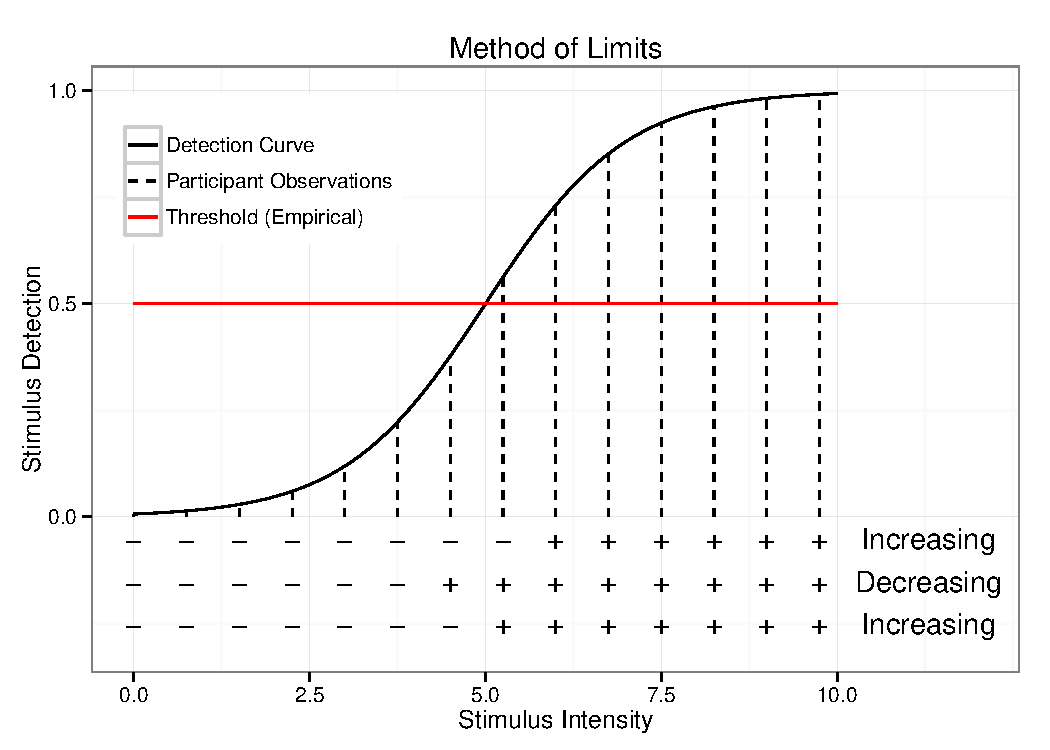
\includegraphics[width=.5\linewidth]{Figure/fig-methodoflimits-1} 

}



\end{knitrout}
\caption[The Method of Limits]{Demonstration of the method of limits. In this experiment, three trials were performed, two trials starting from 0 and increasing, and one trial starting at 9.5 and decreasing. The empirical detection threshold is the threshold at which detection occurs 50\% of the time, and is shown in red. }\label{fig:methodoflimits}
\end{figure}

\paragraph{Method of Adjustment} This method is similar to the method of limits, except that the stimulus intensity is adjusted by the observer (not the experimenter) in a continuous manner until the observer can just barely detect the stimulus. This procedure may be repeated several times, with trials averaged to produce a mean value for the absolute threshold. Figure \ref{fig:methodofadjustment} demonstrates this procedure.
\begin{figure}[htbp]\centering
\begin{knitrout}
\definecolor{shadecolor}{rgb}{0.969, 0.969, 0.969}\color{fgcolor}

{\centering 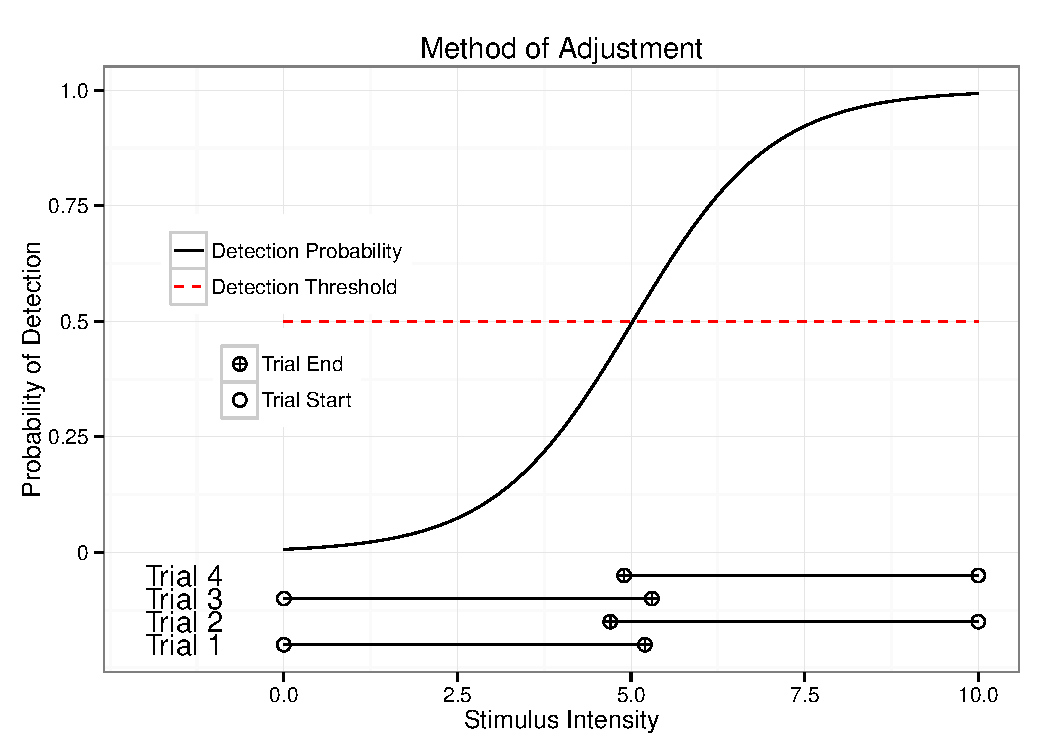
\includegraphics[width=.5\linewidth]{Figure/fig-methodofadjustment-1} 

}



\end{knitrout}
\caption[The Method of Adjustment]{Demonstration of the method of adjustment. In this experiment, four trials were performed, two trials starting from 0 and increasing, and two trials starting at 10 and decreasing. The empirical detection threshold is the threshold at which detection occurs 50\% of the time, and is shown in red. \label{fig:methodofadjustment}}
\end{figure}

\paragraph{Measuring the Difference Threshold} The difference threshold, discussed in section \ref{logarithmicperception}, is the smallest detectable difference between two stimuli. This threshold can be measured using either the method of limits or the method of adjustment. Rather than increasing the absolute intensity of the stimulus as discussed above, two stimuli are given: one with constant intensity and one whose intensity may vary either continuously or incrementally (depending on the method utilized). The participant is instructed to identify the point at which the two stimuli are indistinguishable (if the varied stimulus is approaching the constant stimulus) or the point at which the two stimuli are distinguishable (if the varied stimulus is diverging from the constant stimulus).

\paragraph{Magnitude Estimation} Magnitude estimation studies are used to measure the perceptual intensity of two different stimuli. For example, a participant might be shown a series of two lights, and asked to assign a number to describe how bright each light is. These numerical values would then be compared to the actual light intensity (as measured by a digital sensor or by the input voltage) to determine how perceived brightness corresponds to actual intensity. Many stimuli measured this way produce power-law functions that exhibit response compression (doubling the actual intensity corresponds to a much smaller change in perceived brightness) or response expansion (doubling the actual intensity corresponds to a change in perceived intensity that is more than double the original intensity).

\subsection{Testing Images using Psychological Paradigms}
In addition to the psychophysics methods outlined above, there are testing paradigms within psychology that are applicable to the study of statistical graphics. These include experimental methods such as visual search and eye tracking, as well as experimental control procedures that may be important in graphics studies that are similar to cognitive psychology studies. We will first discuss the experimental methods, and then briefly discuss some common control procedures that may be applicable to the study of statistical graphics.

\subsubsection{Experimental Methods}\label{experimentalmethods}
Many psychological experiments utilize straightforward methods to address hypotheses in perception, such as asking participants to make numerical judgments based on presented stimuli. These methods are quite useful, but not particularly difficult or domain-specific. In this section, we discuss two domain-specific methods for understanding perception of visual stimuli: visual search and eye tracking.

\paragraph{Visual Search} Simply put, visual search methods involve presenting a participant with many distractor stimuli and one or more target stimuli, and asking the participant to locate the target stimuli. Time is measured between the initial stimulus presentation and the participant's answer; participant accuracy is also considered in more complicated visual search settings. This procedure allows researchers to measure simple preattentive stimuli and can also be utilized for more complicated tasks that require attention \citep{anderson1983interactive}. One example of a visual search task is shown in figure \ref{fig:visualsearch}; a common preattentive search task is shown in figure \ref{fig:preattentiveinterference}.

\begin{figure}[htbp]\centering
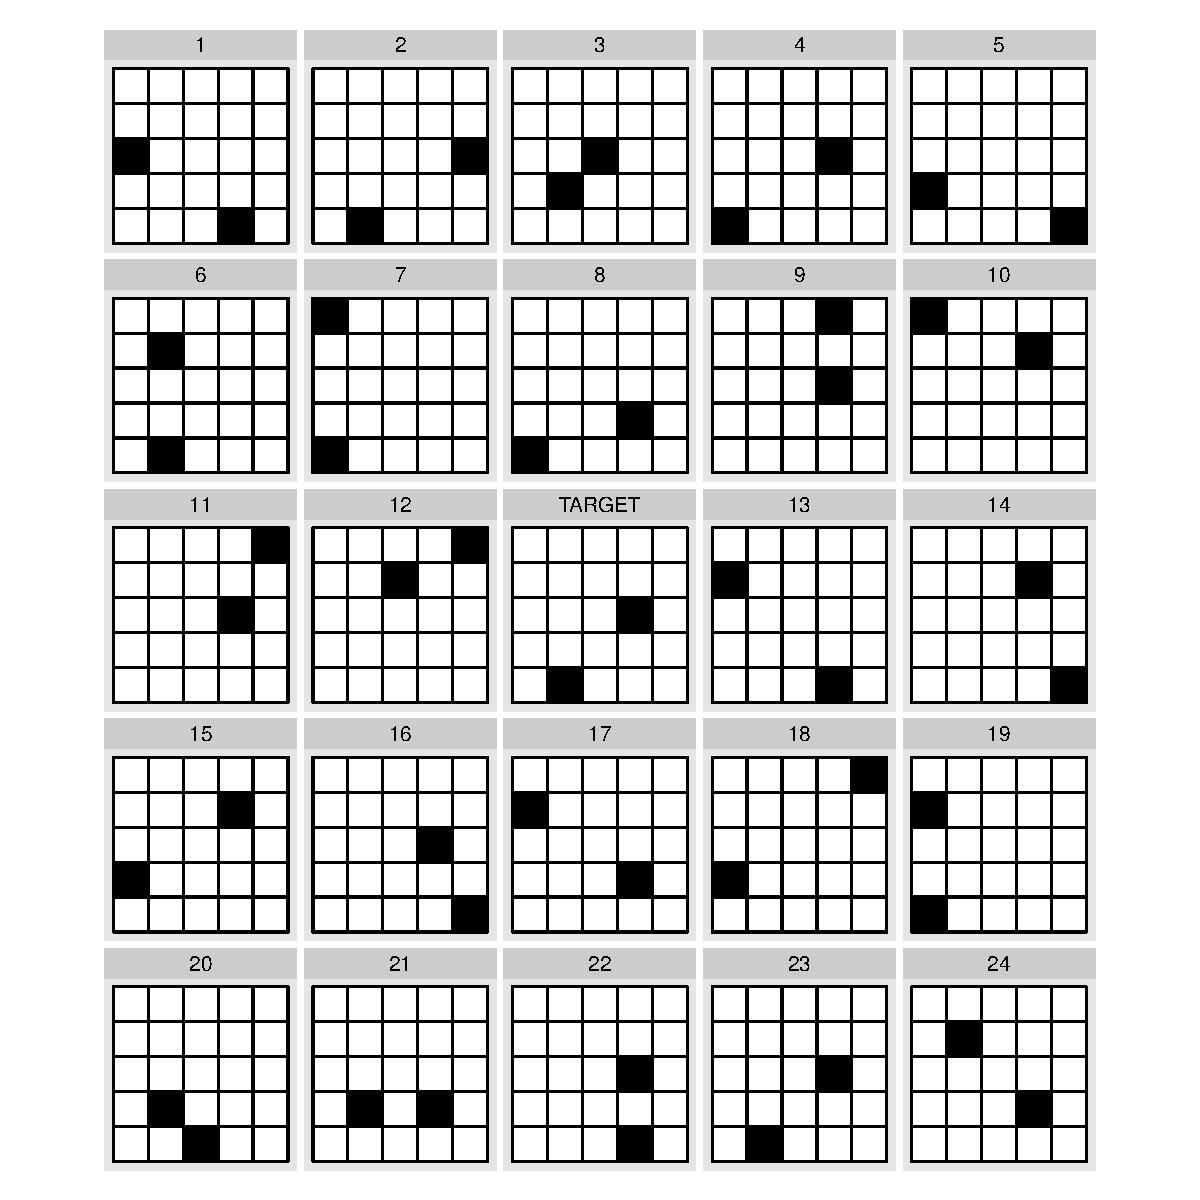
\includegraphics[width=.7\linewidth]{VisualSearch}
\caption[Visual Search Task]{Visual Search Task. Participants were asked to locate the figure (1-24) most similar to the central ``target" figure.}\label{fig:visualsearch}
\end{figure}

Visual search tasks can be used to measure the efficiency of a participant's visual search abilities (and focus on a task) to serve as a baseline for more complicated visual tasks. They can also be used to examine feature binding and common mistakes that may indicate relevant distractor stimuli. Even when reaction time is not directly measured, these tasks are typically given under time pressure, to establish a baseline performance that is below 100\% performance on the task. This time pressure allows experimenters to avoid response compression, so that the number of questions completed within the time limit provides an approximate measure of response time.

\paragraph{Eye Tracking} \label{eyetracking}
Eye tracking studies are often utilized in order to understand which parts or features of an image participants focus on, and in what order they examine the image components. Eye tracking studies were heavily used in order to refine the task-based models of graphical perception; they allowed researchers to understand that participants had to iterate between the question and different parts of the graph in order to assimilate all of the represented information into working memory. Figure \ref{fig:eyetracking} shows one lightweight eye-tracking assembly. The camera allows researchers to track the direction of the pupil and thus infer gaze direction.

\begin{figure}[htbp]\centering
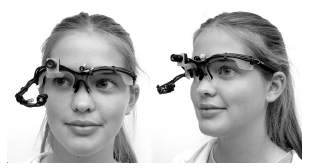
\includegraphics[width=.4\linewidth]{EyeTrackingGear}
\caption[Eye Tracking Equipment]{Eye tracking equipment \protect\citep{babcock2004building}. The cameras allow researchers to determine what part of a scene the wearer is viewing.}\label{fig:eyetracking}
\end{figure}

Eye tracking studies have been performed on statistical graphics as well \citep{zhao2013mind}, utilizing a visual search task and examining which graphics participants compared to determine the target plot.

In some psychological experiments, the straightforward approach to a task can produce biased responses from participants. Human perception is highly reliant on expectations and past experience, and as a result, experimenters must take care to reduce undesired biasing effects in order to appropriately control experiments. Some of these considerations are discussed in the next section.
\subsubsection{Experimental Control Procedures}
While not all of the experimental control procedures discussed here are appropriate for every experiment, they do demonstrate the degree of control many experiments require to measure small psychological effects. The variation in the human brain and in cognitive strategies (and the sample size constraints of testing in humans) requires a large degree of experimental control in order to minimize the effects of population variance. Some of the biases of the human brain as well as strategies to address these biases are described below.

\paragraph{Habituation} The human visual system is attracted to novelty; odd, bizarre, or new sights attract more attention than ordinary, run of the mill scenes. Habituation describes the process of becoming less interested in a stimuli; as this occurs, the mind begins to enter ``auto-pilot" and attention to the task at hand becomes less focused. In infants, this habituation process is used to determine whether there is a perceived difference between two stimuli; in adults, this process is not typically as useful to the experimenter. To avoid habituation, experiments should generally consist of somewhat varied tasks in order to maintain participant attention. The psychophysics experiments described in figures \ref{fig:methodoflimits} and \ref{fig:methodofadjustment} can be vulnerable to this problem; to overcome habituation, trials often alternate in direction or start at random points along the intensity spectrum.

\paragraph{Masking} Images can persist on the retina for a period after the image is no longer available; this phenomenon is called \emph{persistence of vision}. In order to control the time in which the stimulus is visible, psychological experiments often will show a mask immediately after an image in order to ``erase" the retina. This degree of control is often useful in experiments which focus on the preattentive stage of perception, but persistence of vision is not likely to affect experiments which take place in the attentive stage of perception (i.e. images shown for more than .5 seconds). A sample mask is shown in figure \ref{fig:mask}.

\begin{figure}[htbp]\centering
\begin{knitrout}
\definecolor{shadecolor}{rgb}{0.969, 0.969, 0.969}\color{fgcolor}\begin{kframe}


{\ttfamily\noindent\color{warningcolor}{\#\# Warning: Removed 200 rows containing missing values (geom\_point).}}\end{kframe}

{\centering 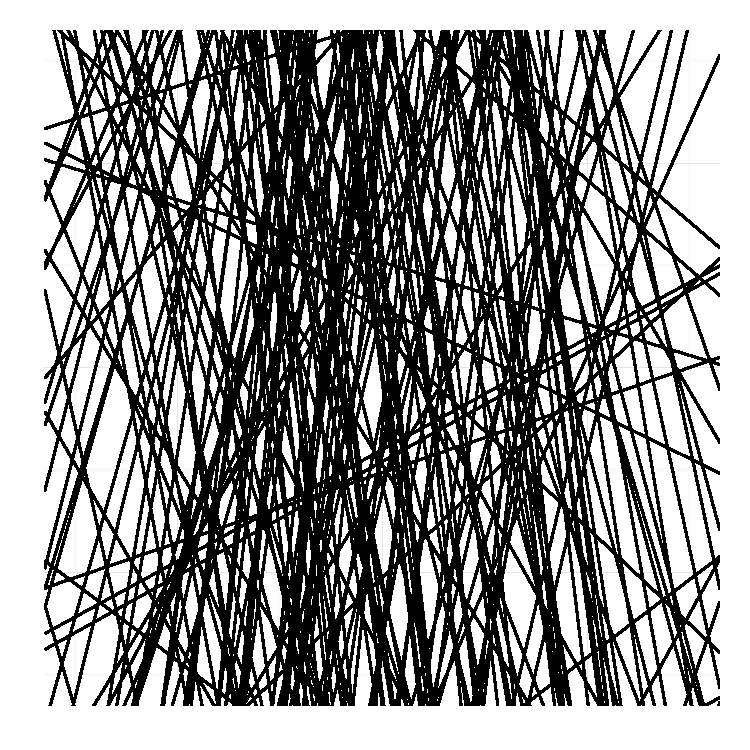
\includegraphics[width=.3\linewidth]{Figure/fig-mask-1} 

}



\end{knitrout}
\caption[Sample Image Mask]{Sample mask used to ``erase'' the retina in some psychological experiments which test stimuli for short time periods ($<$1 s). The mask removes any afterimage the participant might have, ensuring that the stimuli is only available for the specified period. }\label{fig:mask}
\end{figure}

\paragraph{Priming} Broadly, priming is a technique that can be used to subconsciously bias a participant towards a certain conclusion. In cognitive psychology research, priming can be used to test word association (i.e. participants are quicker to identify an apple if they have just heard the word ``fruit" than if they heard the unrelated word ``pen"); in statistical graphics, priming effects are more likely to occur due to instructions or examples provided to participants at the start of a testing session. If an initial example contains notable outliers, participants are more likely to look for and recognize graphs with outliers than graphs with other notable features. Examples must be designed in such a way to avoid activating these priming affects as much as possible.

There are many other psychological mechanisms that may impact participant performance; the mechanisms presented here are simply some of the more salient considerations in experimental design for statistical graphics.

\subsection{Testing Statistical Graphics}
This section details the tools specific to the testing of graph perception within the field of statistics. \citet{cleveland:1985} studied statistical graphics from a largely psychological perspective, but their findings have been widely utilized in the field of statistics; however, it has been 20 years since that paper, and the field has developed within statistics since that time. Two major developments, the grammar of graphics and the lineup protocol, are particularly important for future research into the perception of statistical graphics.

\subsubsection{The Grammar of Graphics}
The grammar of graphics, detailed in \citet{wilkinson2006grammar}, is a framework for describing a graphic in terms of its basic component pieces. An implementation of the grammar of graphics for R, \texttt{ggplot2}\citep{ggplot2, wickham2010layered}, provides a useful tool for manipulating graphics to test in an experimental setting. Using the grammar of graphics, it is easy for experimenters to compare different types of charts using the same data, as the underlying structure of the graph remains the same. Figure \ref{fig:grammarplots} shows three plots created using the same data and different geometric objects, and figure \ref{fig:grammarcode} provides the ggplot2 code to create the plots \footnote{These plots are terrible from a psychological perspective, but serve to illustrate the versatility of the grammar of graphics. In general, stacked density plots, histograms, and dot plots are bad for making numerical comparisons \citep{cleveland:1985}.}. Comparing these graphics experimentally would be reasonably simple, and the grammar of graphics helps to control the extraneous variables introduced by utilizing different plot types. In addition, the grammar of graphics approach to transformations and scales allows us to easily test judgments made utilizing different axis transformations and color scales to compare perceptual accuracy \citep{hofmann2012graphical}.


\begin{figure}[htbp]\centering
\begin{subfigure}[b]{.33\linewidth}\centering
\begin{knitrout}
\definecolor{shadecolor}{rgb}{0.969, 0.969, 0.969}\color{fgcolor}

{\centering 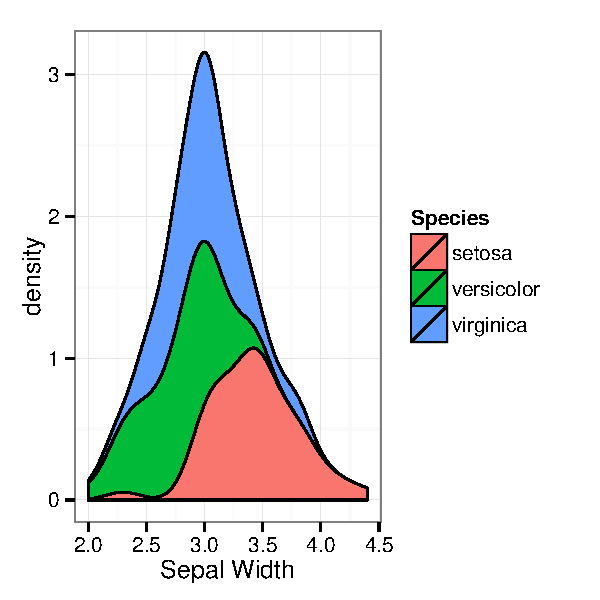
\includegraphics[width=\linewidth]{Figure/fig-irisdatagrammar-a-1} 

}



\end{knitrout}
  \caption{Stacked Density Plot}
\end{subfigure}\hfill
\begin{subfigure}[b]{.33\linewidth}\centering
\begin{knitrout}
\definecolor{shadecolor}{rgb}{0.969, 0.969, 0.969}\color{fgcolor}\begin{kframe}


{\ttfamily\noindent\itshape\color{messagecolor}{\#\# stat\_bindot: binwidth defaulted to range/30. Use 'binwidth = x' to adjust this.}}\end{kframe}

{\centering 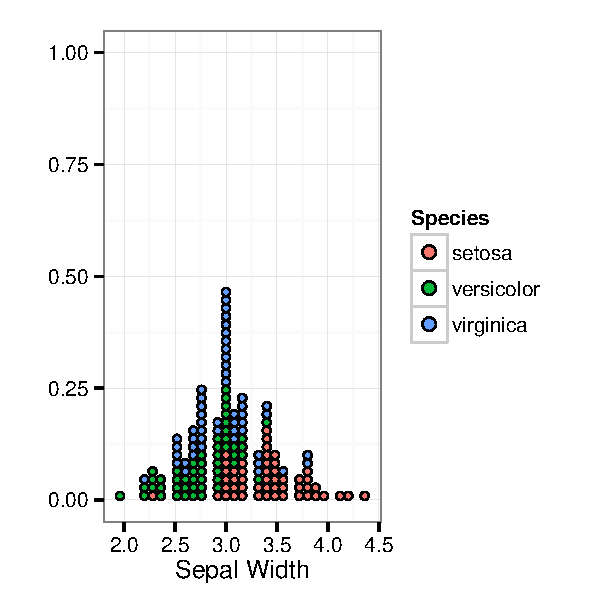
\includegraphics[width=\linewidth]{Figure/fig-irisdatagrammar-b-1} 

}



\end{knitrout}
  \caption{Dotplot}
\end{subfigure}\hfill
\begin{subfigure}[b]{.33\linewidth}\centering
\begin{knitrout}
\definecolor{shadecolor}{rgb}{0.969, 0.969, 0.969}\color{fgcolor}\begin{kframe}


{\ttfamily\noindent\itshape\color{messagecolor}{\#\# stat\_bin: binwidth defaulted to range/30. Use 'binwidth = x' to adjust this.}}

{\ttfamily\noindent\color{warningcolor}{\#\# Warning: position\_stack requires constant width: output may be incorrect}}\end{kframe}

{\centering 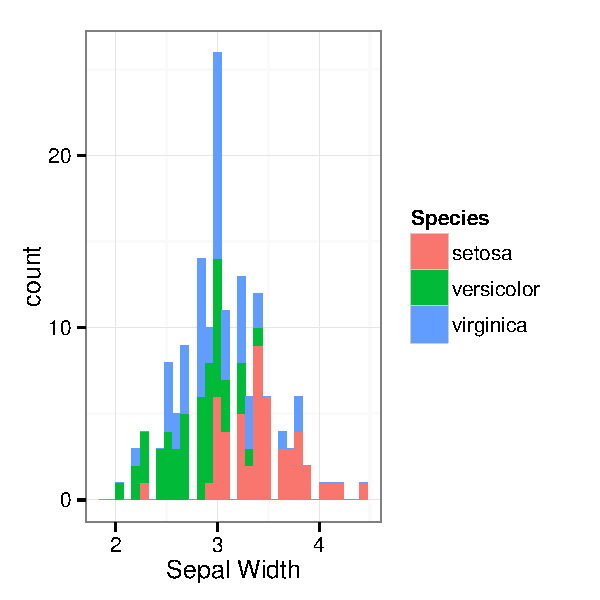
\includegraphics[width=\linewidth]{Figure/fig-irisdatagrammar-c-1} 

}



\end{knitrout}
  \caption{Histogram}
\end{subfigure}\hfill
\caption{Three different plots of iris data, created using the grammar of graphics}\label{fig:grammarplots}
\end{figure}

\begin{figure}[htbp]\centering
\begin{knitrout}
\definecolor{shadecolor}{rgb}{0.969, 0.969, 0.969}\color{fgcolor}\begin{kframe}
\begin{alltt}
\hlcom{# Stacked Density plot}
\hlkwd{ggplot}\hlstd{(}\hlkwc{data}\hlstd{=iris,} \hlkwd{aes}\hlstd{(}\hlkwc{x}\hlstd{=Sepal.Width,} \hlkwc{fill}\hlstd{=Species))} \hlopt{+}
  \hlkwd{geom_density}\hlstd{(}\hlkwc{position}\hlstd{=}\hlstr{"stack"}\hlstd{)}

\hlcom{# Dotplot}
\hlkwd{ggplot}\hlstd{(}\hlkwc{data}\hlstd{=iris,} \hlkwd{aes}\hlstd{(}\hlkwc{x}\hlstd{=Sepal.Width,} \hlkwc{fill}\hlstd{=Species))} \hlopt{+}
  \hlkwd{geom_dotplot}\hlstd{(}\hlkwc{method}\hlstd{=}\hlstr{'histodot'}\hlstd{,} \hlkwc{stackgroups}\hlstd{=}\hlnum{TRUE}\hlstd{)}

\hlcom{# Histogram}
\hlkwd{ggplot}\hlstd{(}\hlkwc{data}\hlstd{=iris,} \hlkwd{aes}\hlstd{(}\hlkwc{x}\hlstd{=Sepal.Width,} \hlkwc{fill}\hlstd{=Species))} \hlopt{+}
  \hlkwd{geom_histogram}\hlstd{(}\hlkwc{position}\hlstd{=}\hlstr{"stack"}\hlstd{)}
\end{alltt}
\end{kframe}
\end{knitrout}
\caption{ggplot2 code to produce figure \protect\ref{fig:grammarplots}}\label{fig:grammarcode}
\end{figure}

\subsubsection{Testing Statistical Graphics using Lineups}
One useful tool for testing statistical graphics is the concept of a lineup. Lineups combine the psychological notion of visual search tasks with the statistical concept of hypothesis testing: Participants are provided with a number of plots of the same form, one using real data and the rest generated using resampling methods. If participants identify the target plot (the plot with real data), this is considered similar in nature to a significant hypothesis test at a given $\alpha$ level (generally, there are 20 plots, so $\alpha=0.05 = 1/20$). Figure \ref{fig:lineupexample} shows a sample lineup.


\begin{figure}[htbp]\centering

\begin{knitrout}
\definecolor{shadecolor}{rgb}{0.969, 0.969, 0.969}\color{fgcolor}

{\centering 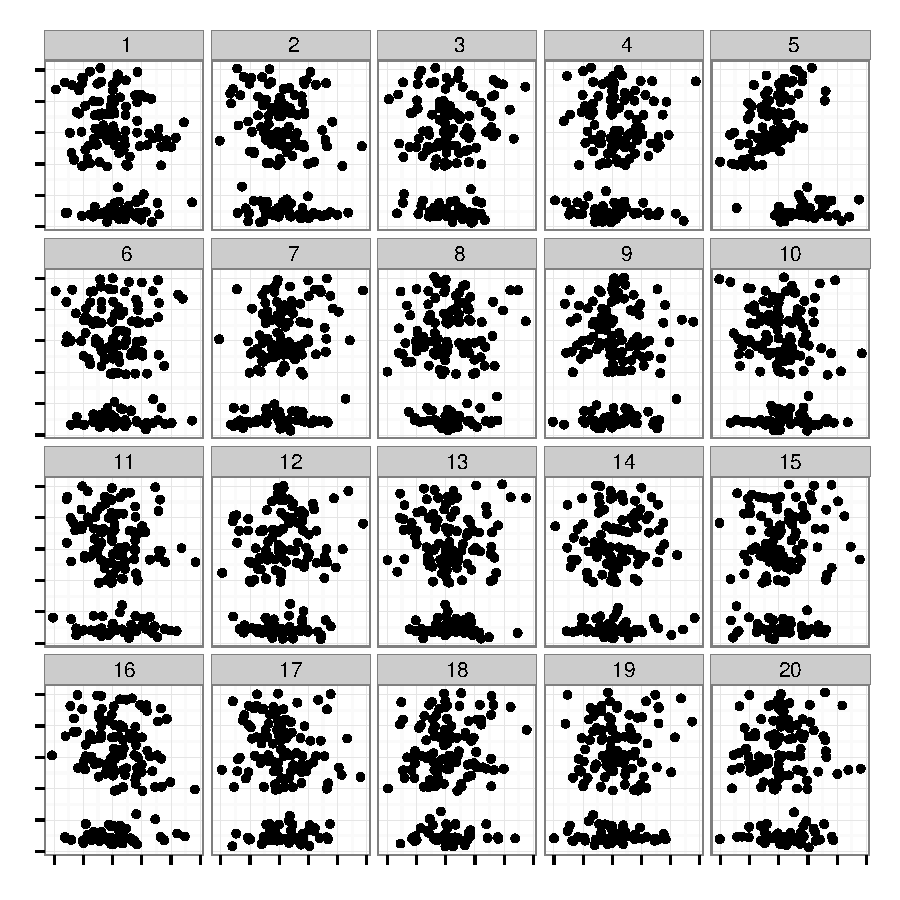
\includegraphics[width=.75\linewidth]{Figure/fig-irislineup-1} 

}



\end{knitrout}
\caption[Lineup for testing statistical graphics]{Lineup of the iris data, comparing sepal width to petal width. The target data is in plot 5, other plots generated by permuting petal width.}\label{fig:lineupexample}
\end{figure}
In addition to the visual inference protocols lineups were designed to fulfill \citep{buja2009statistical}, they also provide a method to easily quantify (on a statistical level) the ``power" of a plot; if two lineups are generated from the same data, but one allows participants to more frequently detect the target plot, then that lineup provides more perceptual power. The lineup protocol provides a useful tool for examining some of the issues discussed for complex, domain specific graphs. When combined with the grammar of graphics approach \citep{wickham2010graphical}, lineups have the potential to be extremely useful for studying the perception of graphs which present the same data in different forms.

\bibliography{../mybib}

\end{document}
